\chapter{Context}\label{chap::1}

\vfill

\minitoc

\newpage

\glsresetall

The application of physics concepts and techniques to the field of health-care is nowadays well-established in the clinical routine. Even if physical techniques have been used in medicine from the earliest time~\parencite{Duck2014}, the discipline today known as \enquote{medical physics} emerged and grown in the past century thanks to the increasing knowledge and use of ionizing radiations both for diagnosis and disease treatment. In the late \nth{19} century, the x-ray discovery by R\"{o}ntgen, the radioactivity discovery by Henri Becquerel, and the radium and radioactive isotopes studies by Pierre and Marie Curie paved the way to the whole medical physics practice of the next century, where x-ray imaging and radiotherapy were soon established. Only three weeks after the discovery of the x-rays, Robert Jones and Oliver Lodge imaged with x-rays a boy's hand~\parencite{Cantor1988}, officially starting the diagnostic application of such a radiation. Following the first successes, more attention were given to radio-protection and dosimetry studies, and the investigations focused on new ways to use radioactive tracers for imaging purpose; this finally led to the birth of nuclear medicine, with the clinical use of the radioisotope \gls{ind131} in 1939~\parencite{Kereiakes1987}. Nuclear medicine rapidly gained importance in the diagnosis clinical panorama, also thanks to the introduction of new detectors, such as the Anger camera introduced in the '60s, and new imaging techniques, such as the detection of photons from positron annihilation (\gls{pet}). Moreover, several alternative methods were proposed or implemented for diagnosis (\gls{mri}, ultrasounds, etc.). In parallel, x-rays were soon employed also for tumor treatment: already in 1896, Emil Grubbe irradiated a woman with breast cancer~\parencite{Evans1951}, and in the same year in Lyon a patient with a stomach cancer has been treated by Victor Despeignes~\parencite{Despeignes1896, Foray2016}. One year later, a skin tumor were successfully irradiated in Vienna using x-rays. Thanks to the invention of the klystron, and, later, of the so-called \enquote{magnetron}, by the Varian brothers with William Webster Hansen, the radiotherapy could spread and become a clinical reality; more refined treatment techniques were then introduced with the development of commercial particle accelerators after World War 2~\parencite{Keevil2012}. 

At present days, the medical physics progress strongly relies on technological development and computer science, which already revolutionized several fields of science. In particular, cancer research is now a key area for technical and technological development, concerning both diagnosis and treatment~\parencite{Webb2009}. Cancer continues to be one of the major issues in the medical scenario: it is at present the second cause of death worldwide, but it is expected to surpass heart diseases and become the main killer in the next tens of years~\parencite{Jemal2010, Thun2010}. The last two decades saw important improvements in radiotherapy techniques and machines, with more precise dose planning and delivery, which enhanced the patient survival and strongly reduced the impact of radiations on healthy tissues. This was possible also thanks to refined imaging technologies, allowing for an accurate tumor volume definition, as well as for image-guided treatments. In this scenario, ion beam therapy, already proposed in the middle of the past century, is rapidly spreading thanks to novel beam delivery technologies, able to relatively reduce the treatment costs and allowing for a commercial diffusion of this treatment method (which is still very limited with respect to standard radiotherapy). Notwithstanding the remarkable steps forward disclosed in the last years, there is still wide room for improvements in this fields, which mainly requires strong imaging basis in order to fully profit of the treatment technique potential.

The work presented in this document have been carried out in this context and mainly deals with the development of gamma imaging detectors to be applied in the field of quality assurance for ion beam treatment. Furthermore, the same detectors have been applied to the nuclear medicine field in simulation, with the aim of assessing its possible clinical implementation for a future development of the nuclear medicine clinical routine. 

In the following sections, a general overview of the two main domains concerned in this thesis work is given. 

\section{Ion beam therapy}\label{chap1::sec::ionBeamTher}
Radiation treatment is an essential component of the tumor therapy, being the second most applied and successful kind of therapy after surgery~\parencite{Schardt2010}. The majority of patiens with localized malignant tumors are treated with radiations~\parencite{Durante2009, Baskar2012, Moding2013}, applied in several fractions in different days in order to reduce the damages to normal tissues~\parencite{Bentzen2006}. The most of the patients treated with radio-therapy techniques receives standard photon treatments, with x-rays coming from linear electron accelerators, while a small percentage undergoes specialized gamma treatments like brachytherapy or gamma knife irradiations. About 1~\% of the radiotherapy patients are irradiated with charged particle beams, with the so-called ion beam therapy~\parencite{Durante2016}.

Ion beam therapy, or \enquote{hadrontherapy}, is a cancer radiation treatment method based on light ion beams instead of photons. It was first proposed by Wilson in 1946 in a famous seminal paper~\parencite{Wilson1946}; the author was asked by its director Ernest Lawrence to clarify the stopping process of protons in matter. Thanks to measurements at the Berkeley cyclotron, he highlighted the physical principles and the possible benefits driven by the implementation of such a kind of radiation in clinical treatments, with particular focus on the simple case of protons and some considerations about heavier ions, like alpha particles and carbon ions.  At that time, the accelerator technologies were still under development after the invention of the cyclotron by Ernest O. Lawrence in 1930, which allowed to increase the range of charged particles in matter, in particular in cells and human tissues, and the treatment required beam energy were about to be reached. Pioneering studies of the biomedical applications of accelerated hadron beams were performed by Cornelius Tobias in 1948~\parencite{Blakely2009} in Berkeley (USA), and the first patients have been treated almost ten years later in the same laboratory by Lawrence and Tobias~\parencite{Tobias1955, Tobias1958} with protons and, later on, with He ions~\parencite{Halperin2006}. New accelerators in four continents were used to continue the quest started in Berkeley, and the experience were extended to carbon ion beams from 1994 in Japan (Chiba), and Germany (Heidelberg - \gls{hit}). 

Nowadays clinical adapted machines are well-established on the market, making ion beam therapy emerging as a wide-spread technique in the every-day cancer treatment routine all over the world. Starting from the early 2000's, many new treatment centers have been designed and built, mainly in Europe and Japan. An intense research effort has been dedicated to this field in the last decades; in addition to considerable improvements achieved in the accelerator technologies, new and refined imaging techniques allowed for important enhancement in the treatment planning, also supported by the continuous development of computer science and the growth of calculation power. In parallel, the biological implications of ion irradiation has been deeply investigated~\parencite{Tobias1982, Brahme2004, Friedrich2012, }. Moreover, since more and more patients are treated every year with this technique, more clinical data are at present available for further study and the connection between physicists and physicians is strongly progressing both in the research field and in treatment practice. Several advancements are expected in the next years, following the extensive research work carried out by several groups in the world. In the following paragraph, the basic physical principles and features of this treatment method are explained, and advantages and drawbacks with respect to standard radiotherapy techniques are analyzed. After that, the need for ion range verification is discussed and detailed in order to reach the main topic for this thesis: the prompt-gamma detection.   

\subsection{Physics of ion beam therapy}\label{chap1::subsec::Physics}
Charged nuclear particle beams at relatively high energy show a characteristic depth-dose distribution in matter which makes them suitable for the application in cancer treatment as a valid alternative to standard photon therapy (x-ray or megavolt beams), bringing several advantages to the patient side. The peculiar energy deposition profile (\enquote{Bragg curve}) is named for Sir William Henri Bragg, who investigated the slowing-down process of $\mathrm{\alpha}$ particles in air~\parencite{Bragg1904, Bragg1905}. 
Low-energy (x-rays) and high-energy photons traversing the patient body deposit their energy by interacting with the target atomic electrons (mainly by Compton interaction), with the deposited dose decreasing at increasing depth after a build-up region (mainly due to forward scattered Compton electrons). Even if the entrance surface (the skin for a patient) can be spared thanks to this build-up region, with a dose peak shift of a few centimeters, a high relative dose is delivered to the tissues along the whole beam path. In order to maximize the tumor volume-to-healthy tissue dose ratio, a standard photon treatment always foresees several irradiation fields from different entrance points and angles (see \figurename~\ref{chap1::fig::XraysCionsFields}, left). This energy deposit behavior is common to all neutral particles, as shown in the first two boxes in \figurename~\ref{chap1::fig::Depth-doseProf} where the depth-dose profiles of photons at various energies and neutrons in water is presented. 
In contrast to neutral particles, the energy deposited per track unit increases for increasing depth for the charged ones: in \figurename~\ref{chap1::fig::Depth-doseProf} the depth-dose profile in water is shown for electrons, pions, protons and neon ions; it is characterized by an entrance low relative dose \textit{plateau} and by a narrow high deposited dose peak at the end of the range (in the last few millimeters), called \enquote{Bragg peak}. The high-dose peak is sharper the more massive is the particle, as clear from \figurename~\ref{chap1::fig::Depth-doseProf}, where the different species are arranged by increasing mass. For what concerns protons and heavier ions, their clinical interest for the treatment of deep-seated tumors appears clear from the above considerations: a nuclear particle beam is able to deliver a reduced dose to the healthy tissues surrounding the target volume, where the dose is concentrated. This allows for the treatment of tumor volumes close to \glspl{oar}, also with limited irradiation angles with respect to photons, as shown in \figurename~\ref{chap1::fig::XraysCionsFields}, right. 

\begin{figure}[!htbp]
\centering
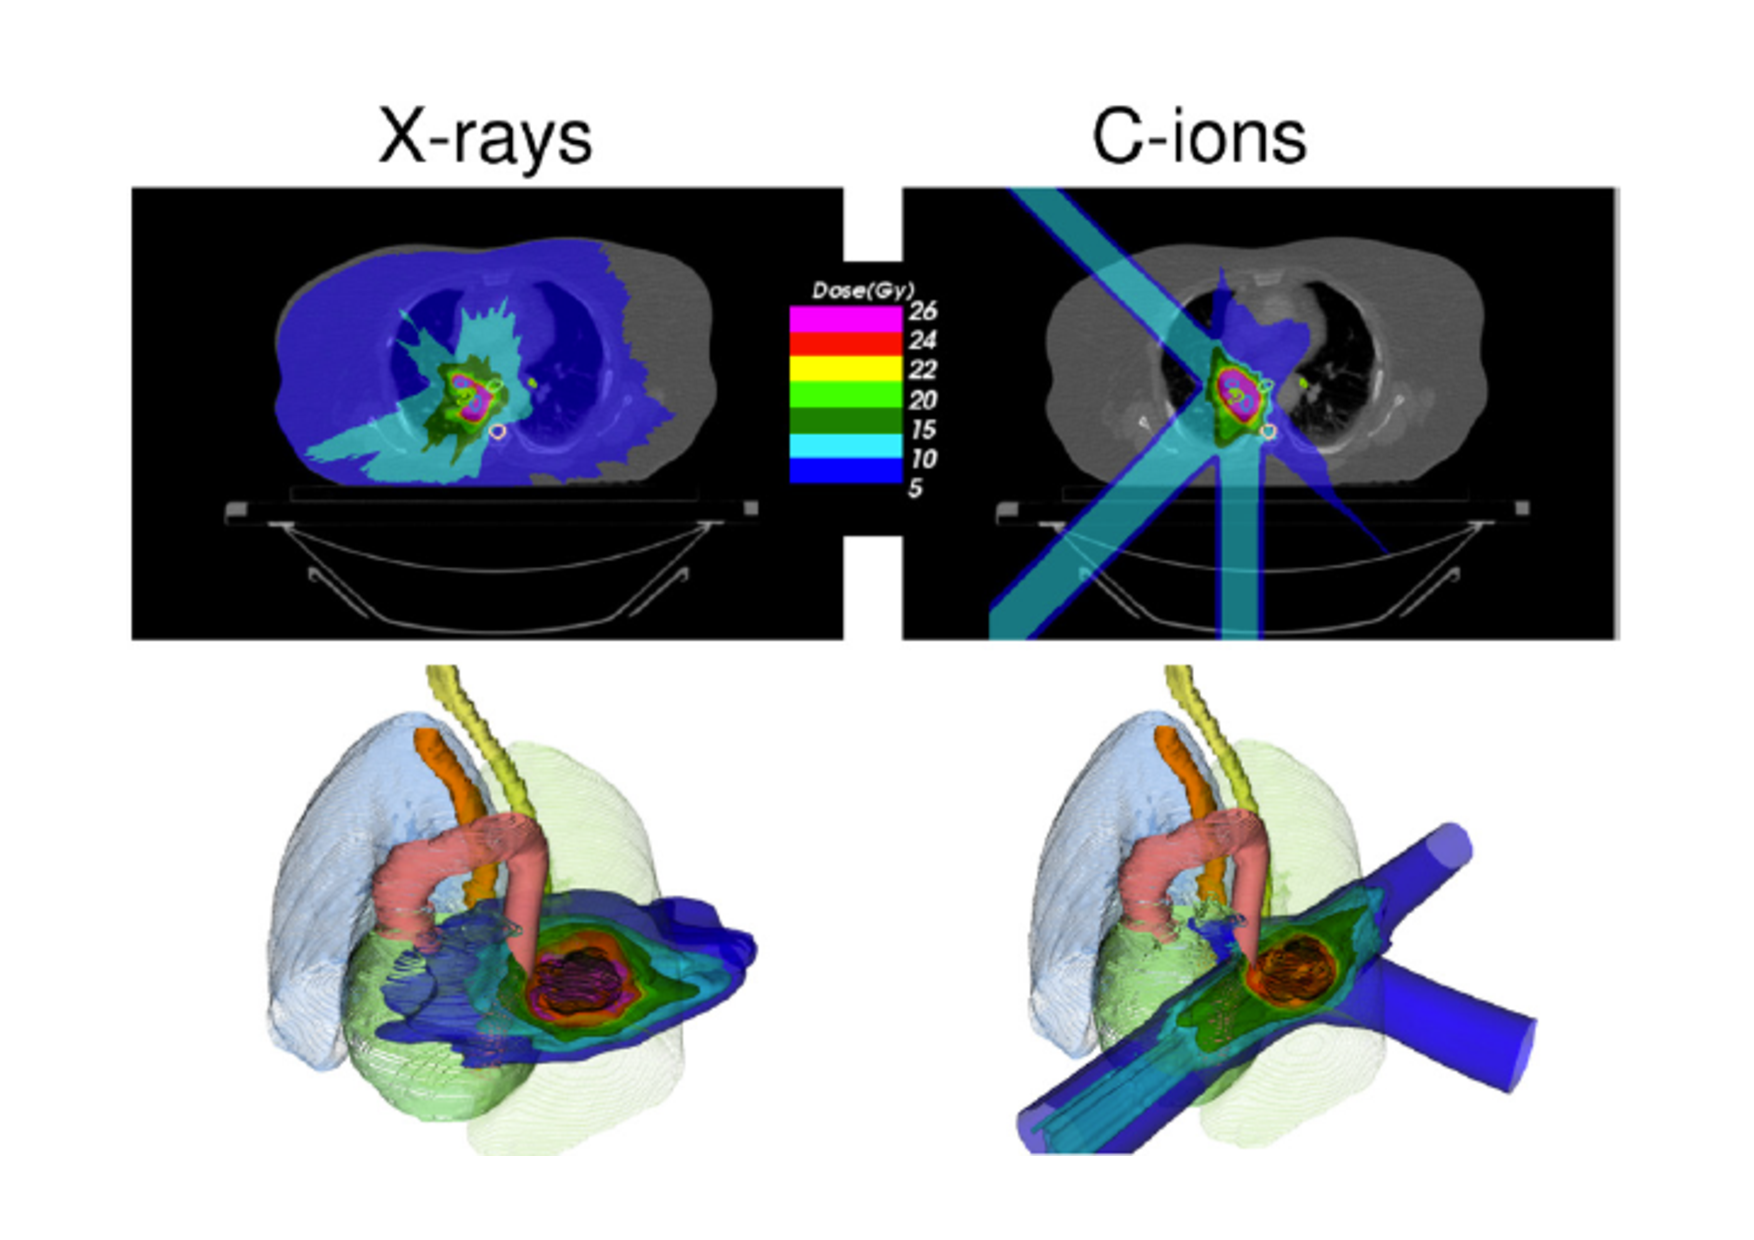
\includegraphics[width=0.6\textwidth]{03_GraphicFiles/chapter1_Introduction/xRayCions_fields.pdf}
\caption{Treatment planning of lung cancer for the irradiation with x-rays (left) or carbon ions (right) (in~\cite{Durante2016}).}
\label{chap1::fig::XraysCionsFields}
\end{figure} 

\begin{figure}[!htbp]
\centering
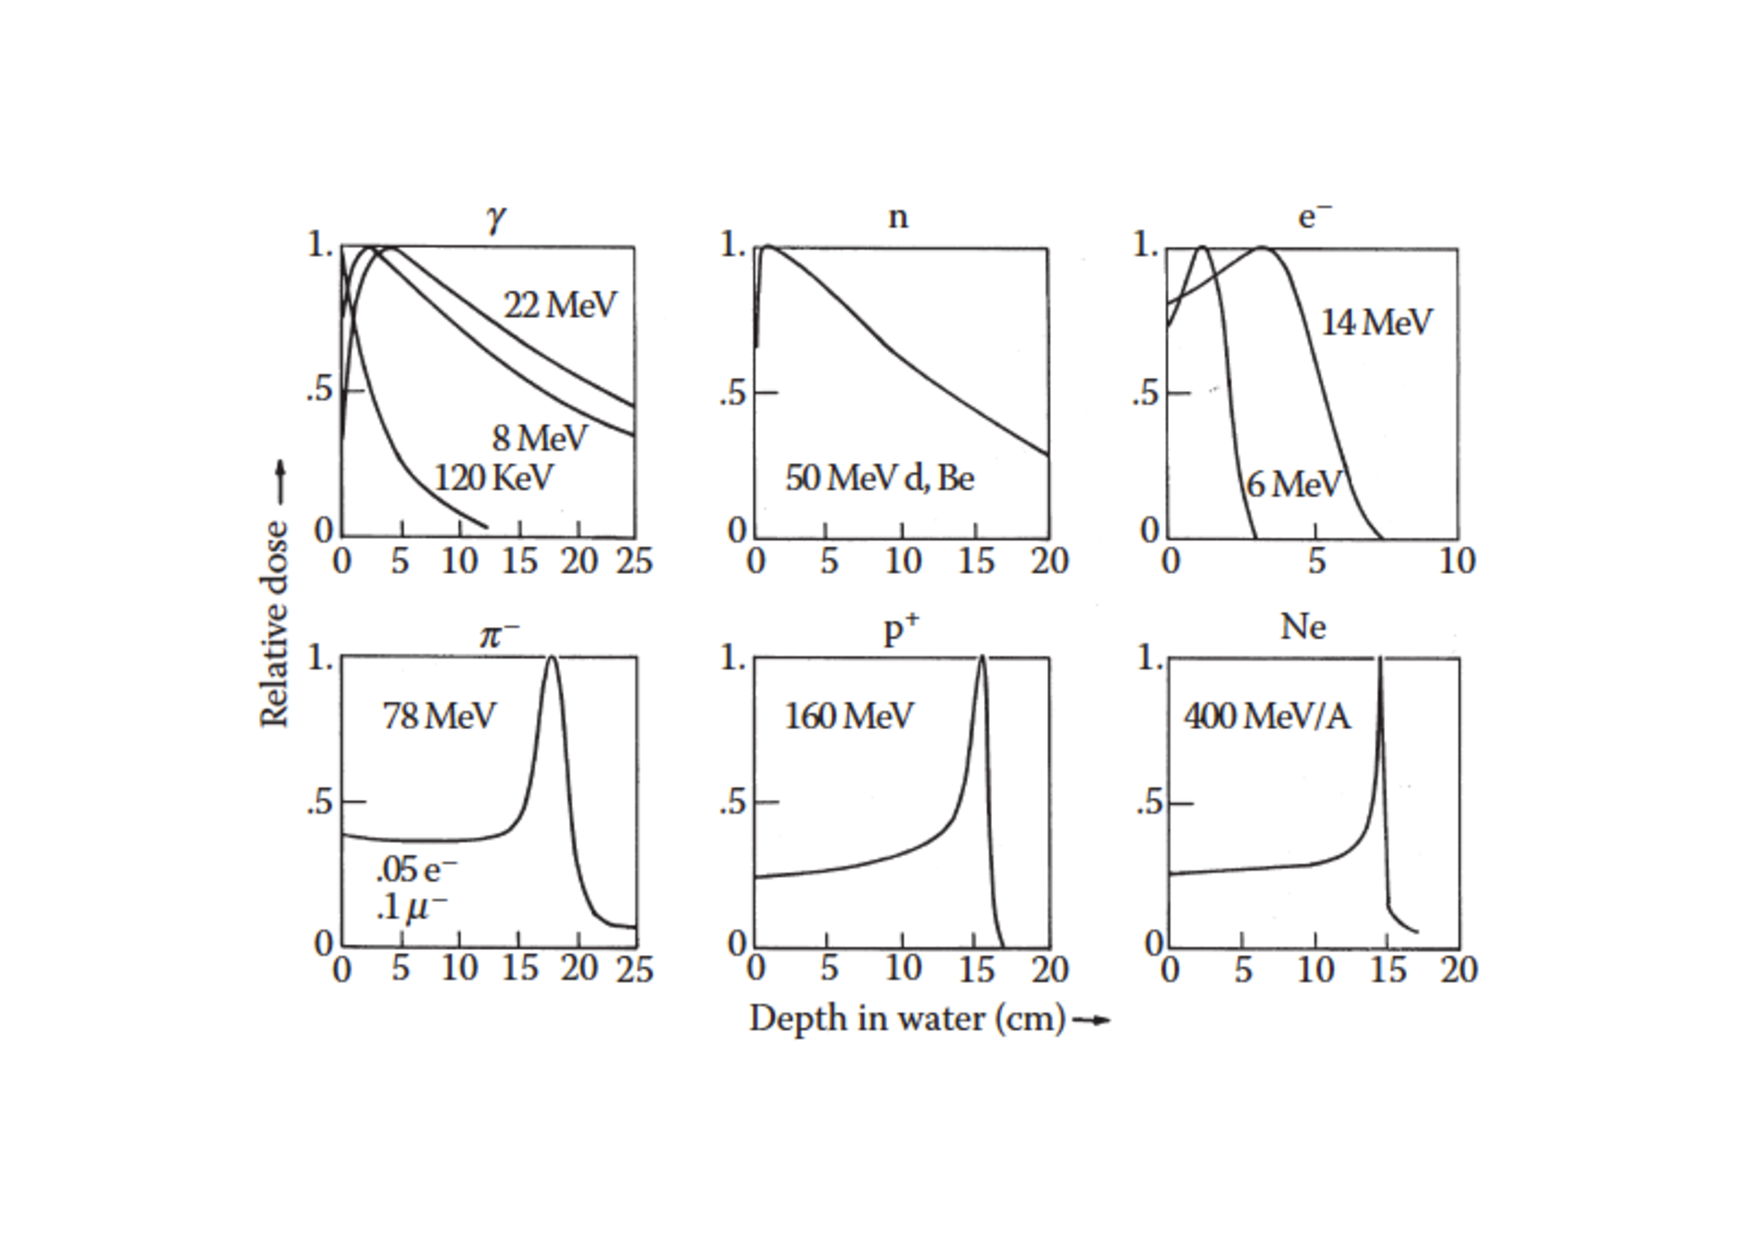
\includegraphics[width=0.7\textwidth , trim={0 0.3cm 0 0.3cm}, clip=true]{03_GraphicFiles/chapter1_Introduction/depth_doseProf_multipleIMG.pdf}
\caption{Relative dose as a function of the particle depth in water for different particle species. In~\cite{PaganettiBook2012}.}
\label{chap1::fig::Depth-doseProf}
\end{figure} 

The nuclear charged particle interactions in matter can be described by three main mechanisms: \gls{em} in-elastic interaction with the atomic electrons, \gls{em} elastic interactions with the atomic nuclei, and nuclear reactions. In addition to the listed interactions, also Bremsstrahlung is theoretically possible, but its effect is negligible at ion energies of clinical interest. 

The \gls{em} in-elastic interactions with atomic electrons cause an energy loss which is generally approximated with a \gls{csda} for simplicity, assuming a mono-dimensional ion path and an average, continuous energy loss rate. This is justified by the mass difference between electrons and ions (as an example, the proton mass is 1832 times greater than that of an electron). The elastic repulsion caused by an atomic nucleus is able to deflect the projectile ion, with an angle which depends on the target-projectile relative mass. The in-elastic nuclear reactions are less frequent, but reduce the intensity of the primary beam (the primary particle is destroyed), and cause the emission of secondary nuclear fragments. A schematic view of the three main interaction mechanisms described is given in \figurename~\ref{chap1::fig::protInteractions} for the example case of protons, while in the following the effects of these interactions are detailed.   

\begin{figure}[!htbp]
\centering
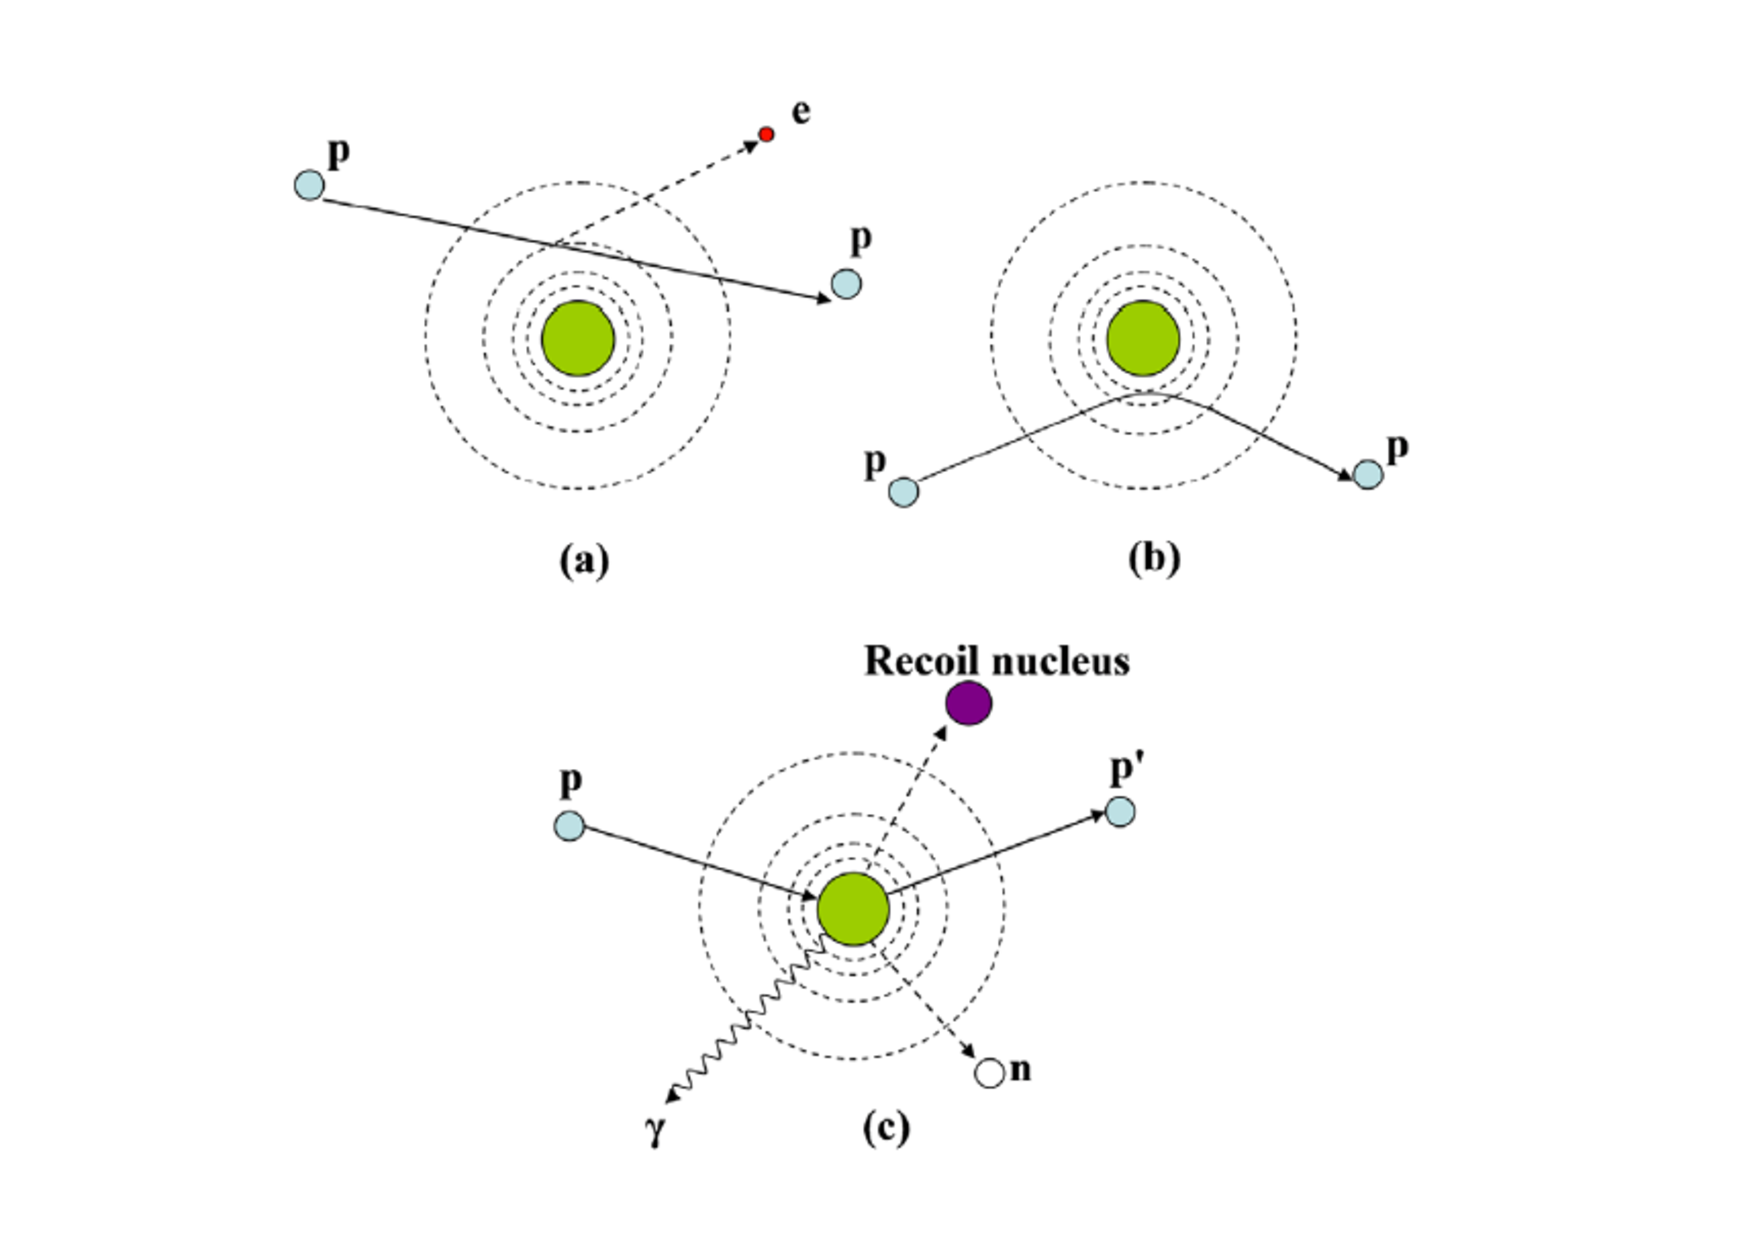
\includegraphics[width=0.7\textwidth]{03_GraphicFiles/chapter1_Introduction/protonInteractions.pdf}
\caption{Schematic view of an example of the three main interactions mechanics of protons in matter: Coulomb interaction with atomic electrons (a), Coulomb interactions with atomic nucleus (b), nuclear reactions(c). In~\cite{Newhauser2015}.}
\label{chap1::fig::protInteractions}
\end{figure} 

At the primary particle velocities of clinical interest,  \myMarginnote{\gls{em} \\ interactions with \\ target atomic electrons} the ion energy loss rate is dominated by in-elastic collisions with the target atomic electorns and is well described by the formula attributed to Bethe~\parencite{Bethe1930} and Bloch~\parencite{Bloch1933}, often referred as Bethe-Bloch formula, reported in equation~\ref{chap1::eq::bethe-bloch} in its form independent of the mass density. This expression is also known as mass stopping power.

\begin{equation}
\frac{S}{\rho} = -\frac{\mathrm{d}E}{\rho \mathrm{d}x} = 4\pi N_{A}r^{2}_{e}m_{e}c^{2}\frac{z^{2}}{\beta^{2}}\frac{Z}{A}\bigg[\ln{\frac{2m_{e}c^{2}\beta^{2}\gamma^{2}}{I}}-\beta^{2}-\frac{\delta}{2}-\frac{C}{Z}\bigg]
\label{chap1::eq::bethe-bloch}
\end{equation}

where $N_{A}$ is the Avogadro's number (6.022 $\times$10$^{23}$mol$^{-1}$), $r_{e}$ is the classical electron radius, $m_{e}$ is the electron mass, $z$ is the charge of the projectile, $Z$ and $A$ are the atomic number and weight of the target material, respectively, $c$ is the speed of light, $\beta = v/c$ is the projectile velocity, $\gamma = (1-\beta^{2})^{-1/2}$, $I$ is the mean excitation potential of the target material. The last two terms represent corrections for high energies ($\delta$ density effect correction term) and low energies ($C$ shell correction term) incident ions. By observing equation~\ref{chap1::eq::bethe-bloch}, it clearly emerges how the energy loss rate is proportional to the inverse square of the projectile velocity and charge. The target material composition also plays a major role. The energy loss rate is directly proportional to the mass density: to be noticed, for clinical applications, that the density in a patient can vary by almost three orders of magnitude, ranging from the air cavity in the lungs to the most dense bones. 
As already mentioned, the energy loss increases for decreasing ion energy due to the $1/\beta^{2}$ dependence, and the maximum energy-loss rate, corresponding to the Bragg peak depth, is reached at the projectile velocity expresses as

\begin{equation}
v_p = z^{2/3}v_{0}
\label{chap1::eq::maxEloss}
\end{equation}

where $v_{0} = e^2/\hslash$ is the Bohr velocity ($\beta$ = 1/137).

The energy loss rate equation directly leads to the definition of the ion beam range in matter (if we neglect nuclear interactions which cause a modification of the projectile nature), which is the integral over the incident energy of the energy loss per track unit, reported in equation~\ref{chap1::eq::rangeIntegral}. This formulation assumes a 1D ion trajectory with negligible lateral scattering (discussed below) and uses the \gls{csda}. 

\begin{equation}
R(E) = \int_{0}^{E}(\frac{\mathrm{d}E'}{\mathrm{d}x})^{-1}\mathrm{d}E' 
\label{chap1::eq::rangeIntegral}
\end{equation}

E is the ion beam incident energy. To be noticed that the range is not a deterministic value, but it is intended as an average value and defined for the whole beam, not for single incident particles, which are affected by statistical fluctuations in the energy loss, leading to the so-called range straggling (described by different theoretical models, such as the ones in~\cite{Bohr1915, Landau1944, Vavilov1957}, and detailed below). Integration of the Bethe-Bloch is often a hard task, but, as realized by Bragg and Kleeman~\parencite{Bragg1905}, the range dependence on the incident particle energy can be practically expressed with an analytic approach as the power law in equation~\ref{chap1::eq::rangePowerLaw}. This approximation directly derives from studies on alpha particles which anticipated the formulation of equation~\ref{chap1::eq::bethe-bloch}.

\begin{equation}
R(E) = \alpha E^{p}
\label{chap1::eq::rangePowerLaw}
\end{equation}

E is again the ion beam initial energy, the constant $\alpha$ depends on the target material and the constant $p$ is related to the projectile energy (or velocity). The proton range can be easily scaled to other ions at the same energy per nucleon in the same material with a factor $M/z^{2}$. The range of ions with the same specific energy scales from water to other homogeneous material with a factor of $A/Z^{2}$.
%An empirical expression has been derived to scale the proton calculated range to heavier ions at the same energy per nucleon in the same material: it is reported in equation~\ref{chap1::eq::ScaleRange}.

%\begin{equation}
%\frac{R_{2}}{R_{1}} = \frac{M_{2}}{M_{1}}\frac{z_{1}^{2}}{z_{2}^{2}}
%\label{chap1::eq::ScaleRange}
%\end{equation}

%with M and z the ion mass and charge, respectively. Equivalently, for the same particle in different material, the scaling formula is reported in equation~\ref{chap1::eq::ScaleRangeMat}.

%\begin{equation}
%\frac{R_{2}}{R_{1}} = \frac{\rho_{2}}{\rho_{1}}\frac{\sqrt{A_{1}}}{\sqrt{A_{2}}}
%\label{chap1::eq::ScaleRangeMat}
%\end{equation}
 
% with $\rho$ and $A$ density and atomic mass of the target material, respectively.
 
The ion range predicted by equations~\ref{chap1::eq::rangeIntegral} or~\ref{chap1::eq::rangePowerLaw} is an average value, calculated by considering a smooth and continuous energy loss process and neglecting the individual ion features paths. The actual range suffers from statistical fluctuations in the primaries initial energy and energy loss that broaden the Bragg peak, in the so called \enquote{range straggling}. In general, the longitudinal beam straggling can be described by an asymmetric distribution~\parencite{Vavilov1957}, which is approximated to a Gaussian in the limit of many collisions, leading to the expression of the relative straggling in equation~\ref{chap1::eq::relStragg}:
 
 \begin{equation}
\frac{\sigma_{R}}{R} = (M^{-\frac{1}{2}})\phi\frac{E}{Mc^{2}}
\label{chap1::eq::relStragg}
\end{equation}

The ratio of the straggling width $\sigma_{R}$ and mean range $R$ is then all the more reduced as the ion mass ($M$) increases, with $\phi$ a slowly varying function which depends on the target material~\parencite{Rossi1952} and E the ion energy. According to equation~\ref{chap1::eq::relStragg}, it is interesting to notice how the relative straggling for carbon ions is about 3.5 times smaller with respect to protons (e.g. 7~mm and 25~mm at 18~cm of average range for carbon ions and protons, respectively - see~\cite{Durante2016}).

In addition to the energy loss process considered till here,  \myMarginnote{\gls{em} \\ interactions with \\ target nuclei} which shapes the beam in the longitudinal direction (range variations), the actual delivered dose also depends on the lateral beam profile, which is mainly governed by elastic Coulomb scattering with atomic nuclei and by secondary particles produced by nuclear fragmentation. 
In case an ion passes close to a target atomic nucleus, it is elastically scattered by the repulsive electromagnetic force: the projectile loses a negligible amount of energy, so that this kind of interaction can be neglected when calculating the energy loss rate described above, but the change in its trajectory must be estimated for range and dose predictions. %The \gls{mcs} is determined by elastic electromagnetic interactions of the beam ions with the target nuclei, causing considerable deflections in the single ion trajectory which mainly affect the lateral beam profile causing a spread. 
Starting from the single scattering model by Rutherford~\parencite{Rutherford1911}, and moving to the calculation of the statistical distribution function for the scattering angle at a certain penetration depth given by~\cite{Bothe1921}, a complete theory allowing for the calculation of the scattering angle probability in case of \gls{mcs} has been proposed by Moli\`{e}re~\parencite{Moliere1948} (confirmed to provide good predictions thanks to a large set of proton beam spread data - see~\cite{Gottschalk1993}). %and then simplified for analytic calculations towards a Gaussian approximation. %The Gaussian standard deviation expression in equation~\ref{chap1::eq::latSpread} is given by the characteristics \gls{mcs} angle~\parencite{Highland1975}

% \begin{equation}
%\sigma_{\theta} = \frac{14.1 \mathrm{MeV}}{\beta p c}Z_{p}\sqrt{\frac{L}{L_\mathrm{rad}}}\big[1+0.038 \ln\big(\frac{L}{L_{\mathrm{rad}}}\big) \big]
%\label{chap1::eq::latSpread}
%\end{equation}

%where $L$ is the material thickness and $L_{\mathrm{rad}}$ is the radiation length (reported for common materials in~\cite{Tsai1974}). 
%Even if the Gaussian approach is not always accurate to describe the lateral beam spread (mainly at large angles), 
The Moli\`{e}re \gls{mcs} description allows to retrieve the main parameters contributing to this effect: in particular, heavier particles have more narrow lateral beam shape, and the scattering effect increases at increasing ion range (but is inversely proportional to the beam energy) and for high-Z materials. A more precise model of the lateral beam spread should involve nuclear reactions and the produced secondary particles, but an analytic approach is difficult and Monte Carlo based calculations are still time consuming. The empirical parametrizations are still strongly based on experimental data: as an example, measurements of the lateral beam spread in a water column for different beam energies (ranges) are reported in~\cite{Pedroni2005}.  

In addition to the electromagnetic interactions with electrons and nuclei \myMarginnote{Nuclear reactions}  which mainly govern the stopping process, primary ions impinging on a target also undergo nuclear reactions with the target nuclei which may cause the disintegration of the projectile and the target nucleus or a partial fragmentation. In general, nuclear reactions induce modifications in the beam composition and cause variations in the longitudinal and lateral beam structure which must be taken into account for the delivered physical and biological dose estimate. Moreover, this kind of reactions leads to the production of secondary particles, such as secondary protons, neutrons, hydrogen and helium isotopes and other ions (mainly with heavy ion irradiation), and gammas.

The nuclear interactions occurring between projectile ions and target nuclei can be described by a two-step process. At the \enquote{collision} stage, depending on the distance between projectile and target centers (impact parameter $b$), a variable number of nucleons is involved in the interaction and composes the reaction zone generally defined \enquote{fireball}. The so-called \enquote{spectator} nucleons are almost not affected and create projectile and target-like fragments (\enquote{fragmentation} process), often in excited states . After the collision, the excited fireball and fragments decay through the emission of secondary light particles, in the so-called \enquote{de-excitation} process, and the lighter fragments continue their path through the target. A schematic view of a typical nuclear reaction is given in \figurename~\ref{chap1::fig::nuclReac}. 
Several models have been proposed to describe the two steps, and a complete description of the overall process is given by the so-called abrasion-ablation model~\parencite{Serber1947, Hufner1975} generally used in therapy transport codes, where the abrasion phase describes the collision and the ablation one models the de-excitation stage. To be noticed that the ablation description is more adapted to peripheral collisions (high $b$), where the fragments are excited after the collision and decay to the ground state by emitting light particles and gamma rays.%, depicted in \figurename~\ref{chap1::fig::abrAbl}.

\begin{figure}[!htbp]
\centering
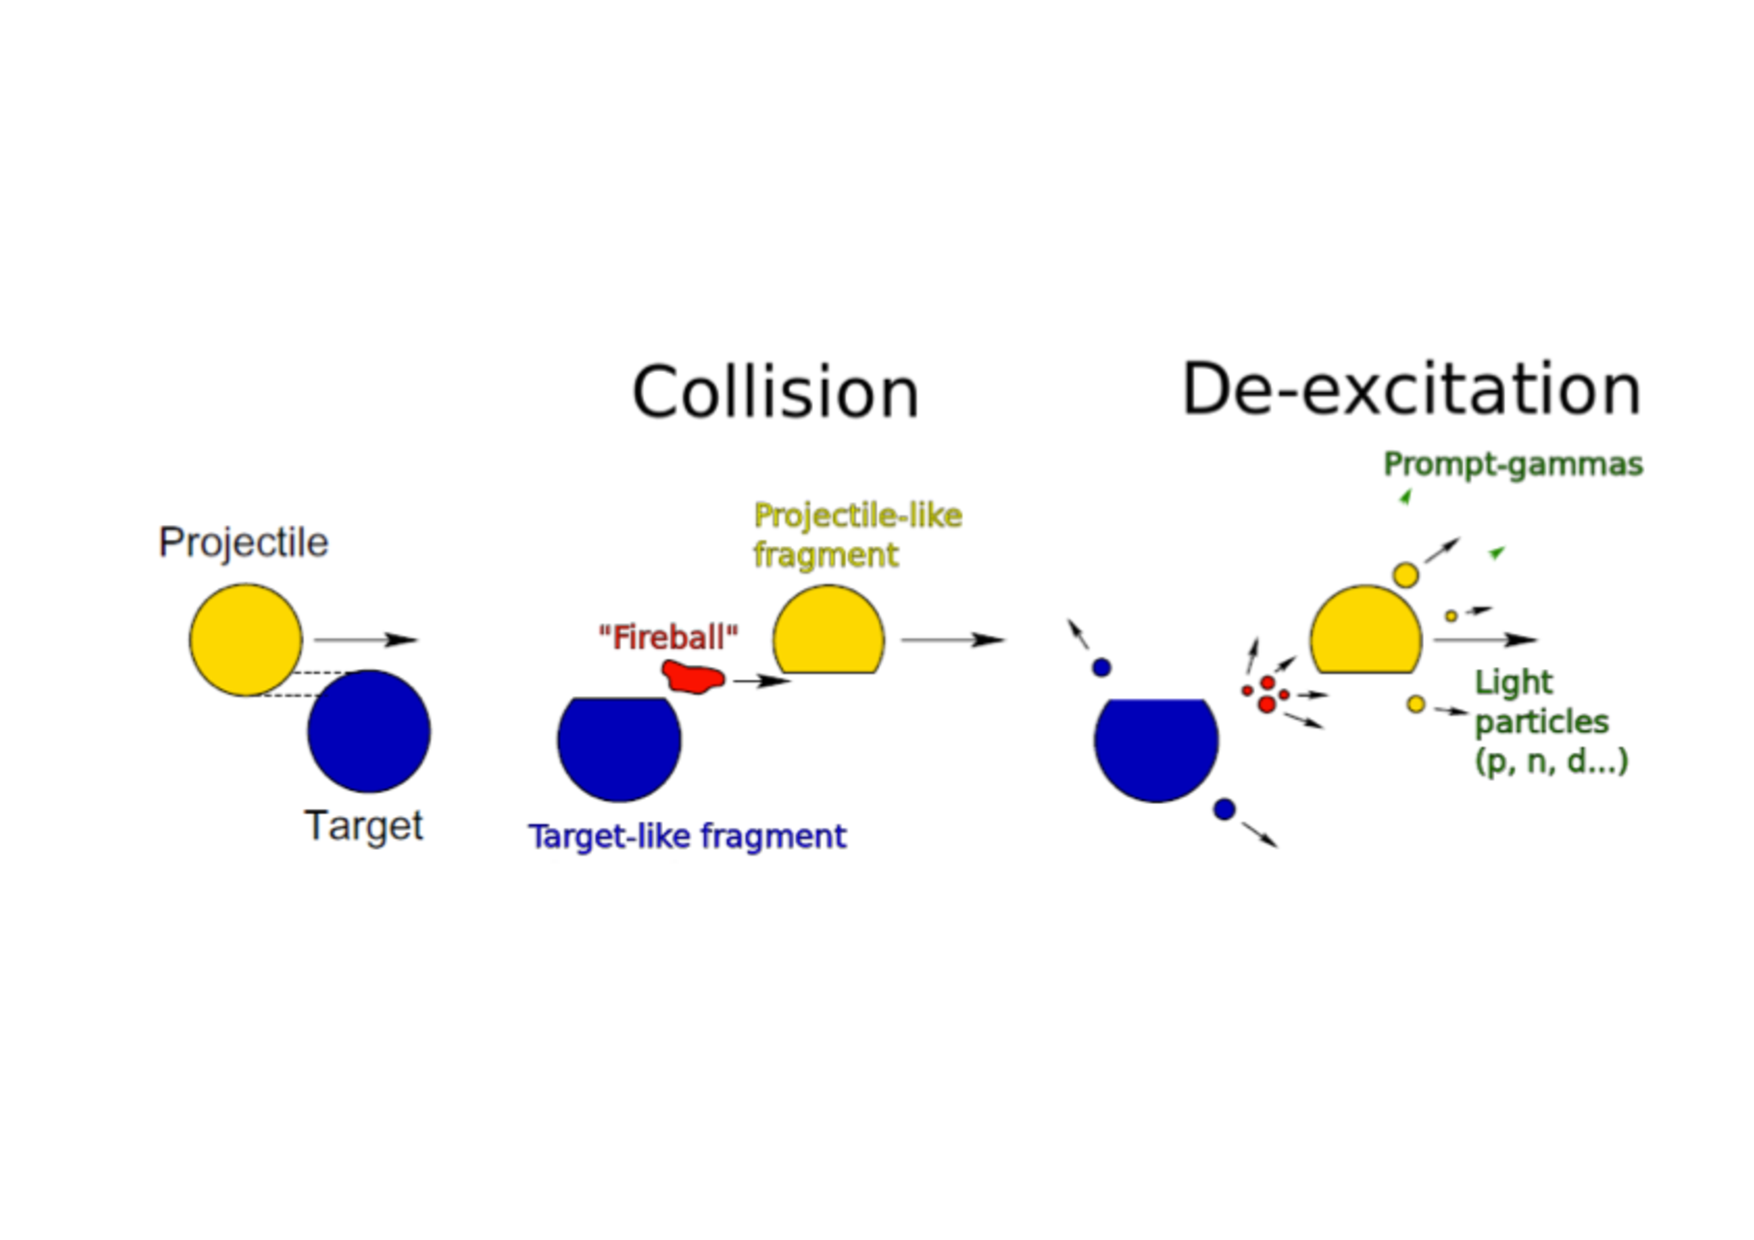
\includegraphics[trim={0 5cm 0 3cm} , clip , width=0.95\textwidth]{03_GraphicFiles/chapter1_Introduction/nuclReactionsScheme.pdf}
\caption{Schematic view of the nuclear reaction between a projectile and a target nucleus. The two steps are defined as \enquote{collision} and \enquote{de-excitation} processes.}
\label{chap1::fig::nuclReac}
\end{figure} 


%\begin{figure}[!htbp]
%\centering
%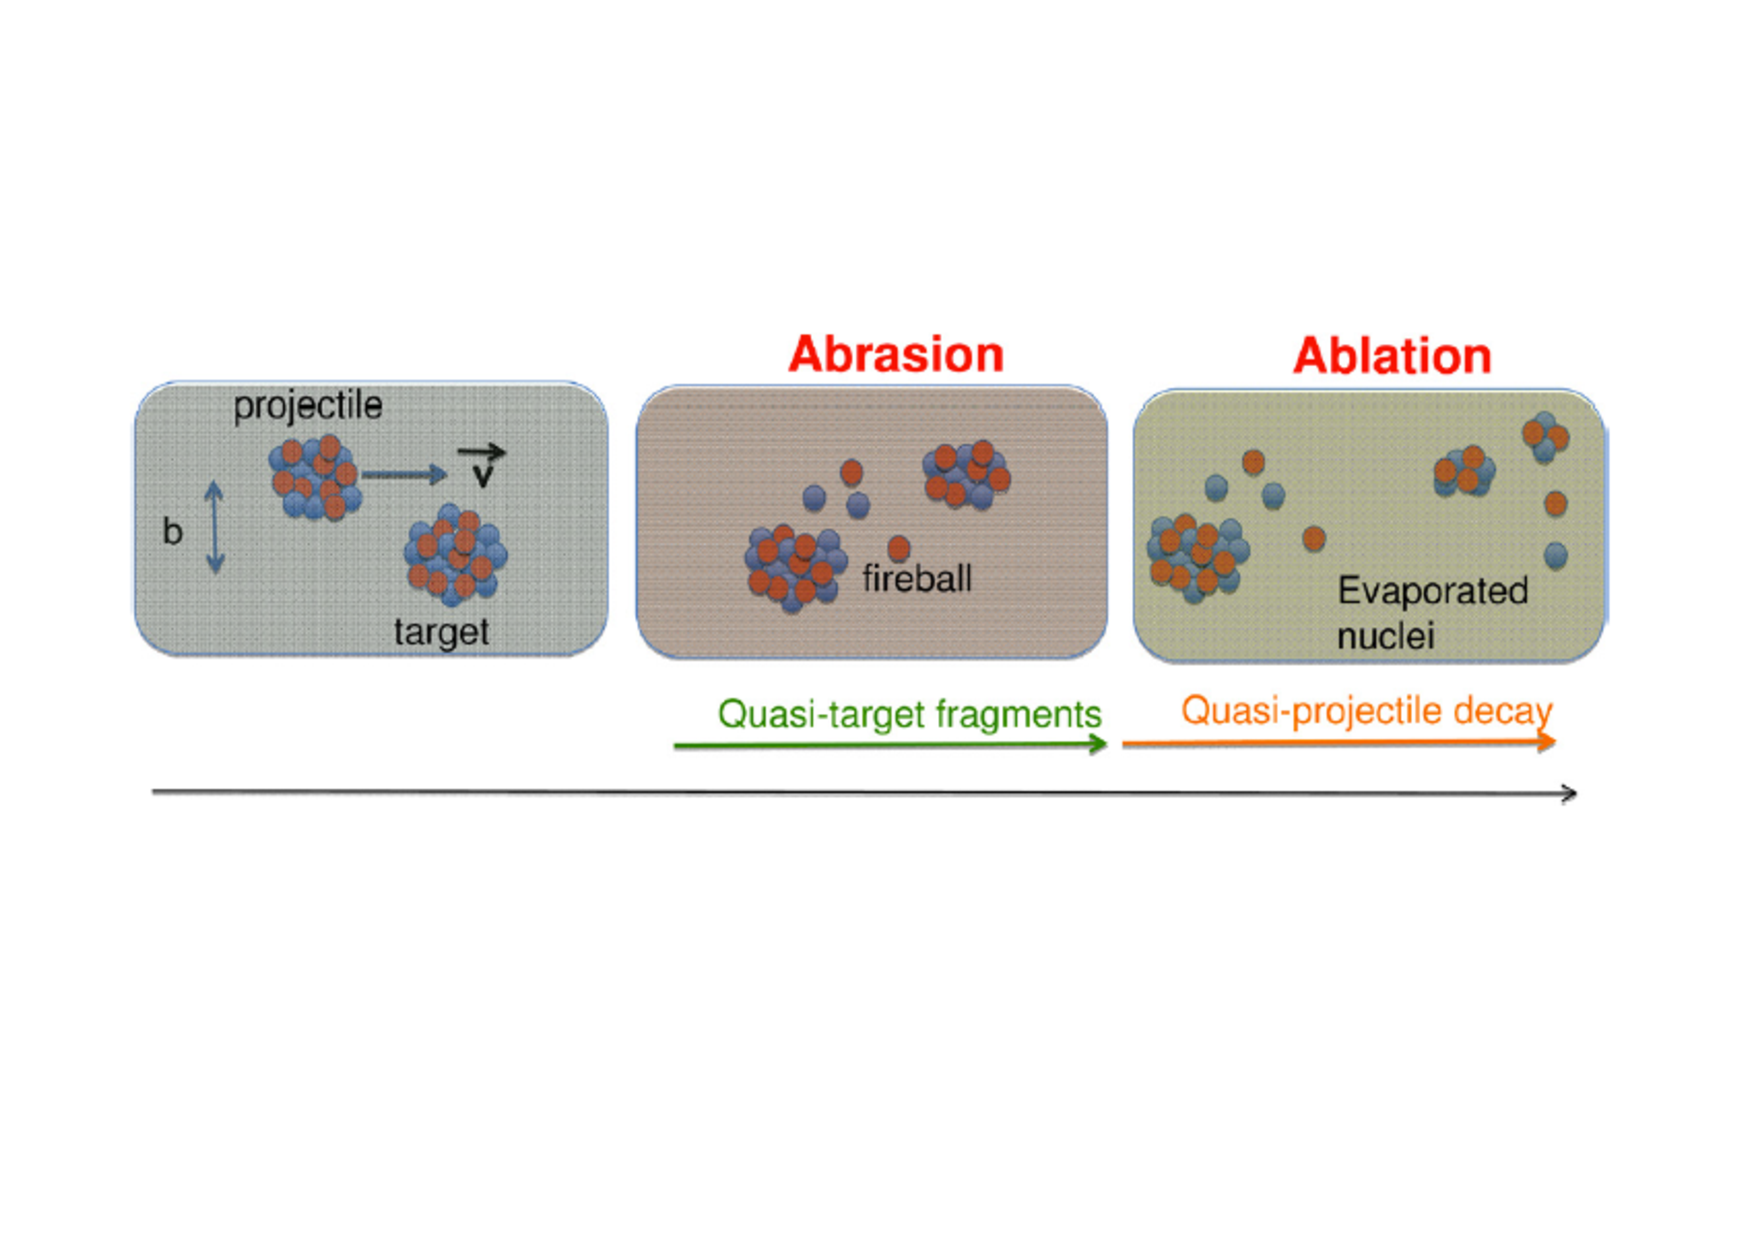
\includegraphics[trim={0 5cm 0 3cm} , clip , width=0.95\textwidth]{03_GraphicFiles/chapter1_Introduction/AbrasionAblation.pdf}
%\caption{Schematic view of the abrasion-ablation model for the description of ion-nucleus interactions (in~\cite{Durante2016}): b is the impact parameter, v is the projectile velocity.}
%%\end{figure} 

Two main effects of fragmentation processes are relevant to ion beam therapy. 
First, the described nuclear reactions cause a loss of primary beam particles; this effect is all the more important for increasing penetration depth. It is clear that peripheral collisions (high $b$) lead to smaller loss of primaries with respect to central collision (small $b$), where projectile and target are most likely completely destroyed. \figurename~\ref{chap1::fig::nuclearReacLoss} shows the primary particle fluence loss in a proton beam as a function of the depth in water~\parencite{Newhauser2015}. In the entrance region before the falloff the fluence loss is caused by nuclear reactions, while close to the Bragg peak the fluence falloff is mainly due to absorption of primary particles with limited residual energy. In addition, the range straggling effect is visible. Concerning carbon ion beams, as reported in~\cite{Durante2016}, during a standard treatment only 50\% of the primary ions reaches the Bragg peak region, while the others undergo fragmentation processes and are lost.
Second, lower-mass and Z fragments result from the nuclear interactions in case of irradiation with ions heavier than protons (with proton beams, only secondary protons and neutrons are produced).
The projectile velocity determines the velocity of the secondary fragments, which can travel with longer ranges with respect to the primaries due to their reduced mass and charge (remember the range scaling factor $M/z^{2}$): this produces a tail in the dose distribution (for ions heavier than protons). The features of this tail have been deeply studied for different primary ions species ($^{10}$B, $^{12}$C, $^{14}$N, $^{16}$O, $^{20}$Ne), and shell-structure effects have been verified with a non-direct relationship between proton number Z and tails extension~\parencite{Schall1996}.  \figurename~\ref{chap1::fig::TailBragg} show the effects of nuclear reactions on the Bragg curves related to carbon ion beams at different energies stopping in water, measured in a water column~\parencite{Schardt2008}.  With increasing primary energy and, consequently, beam penetration depth, the ratio between Bragg peak and entrance plateau dose is reduced by the decreased number of primary ions, while the tail after the Bragg peak is wider due to the increased number of lower-Z fragments traveling with longer range. In addition to this, the energy loss stochastic fluctuations is clearly visible in the broadening of the Bragg peak.  

\begin{figure}
\begin{subfigure}[t]{.49\textwidth}
\centering
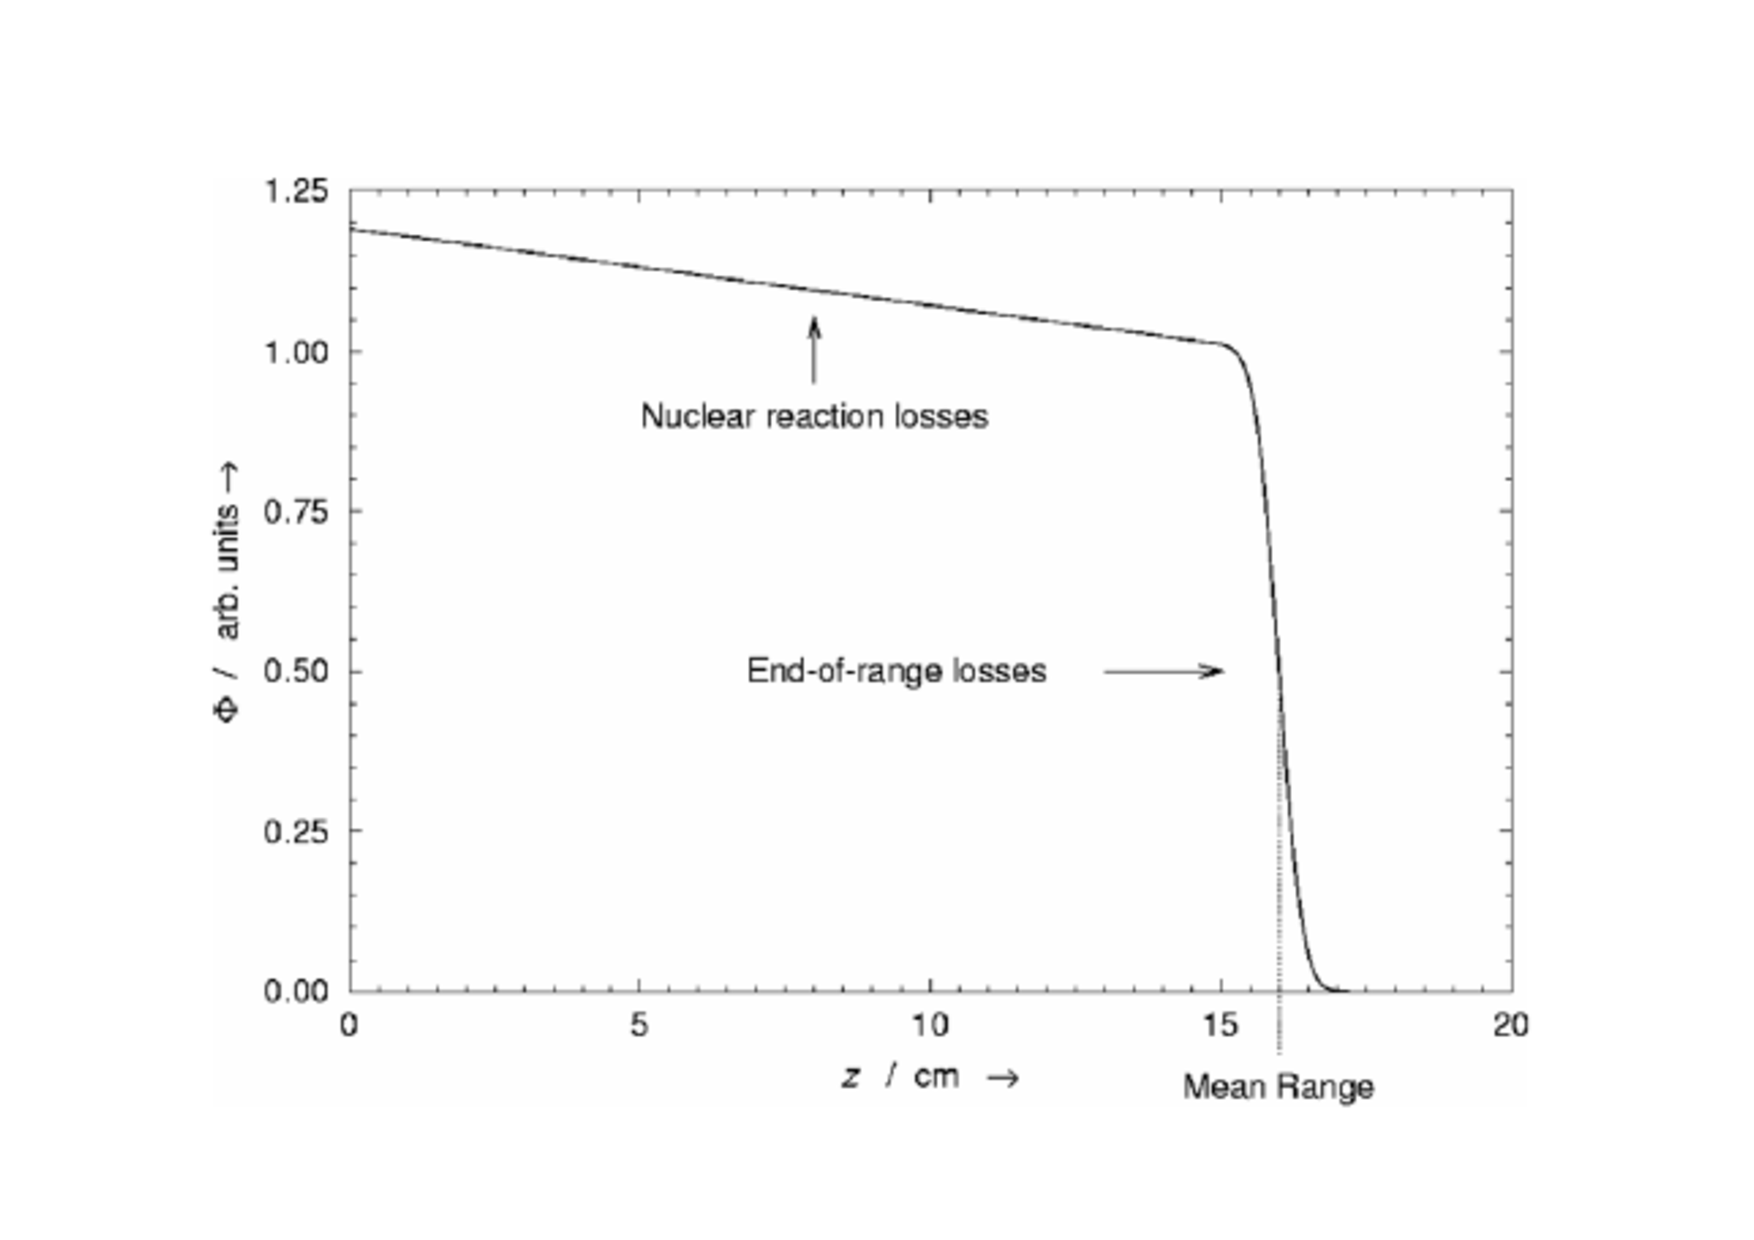
\includegraphics[width=0.99\linewidth]{03_GraphicFiles/chapter1_Introduction/primaryLoss.pdf}
\caption{Primary particle fluence loss in a pro\-ton beam as a function of the depth in water (in~\cite{Newhauser2015}).}
\label{chap1::fig::nuclearReacLoss}
\end{subfigure}
\begin{subfigure}[t]{.49\textwidth}
\centering
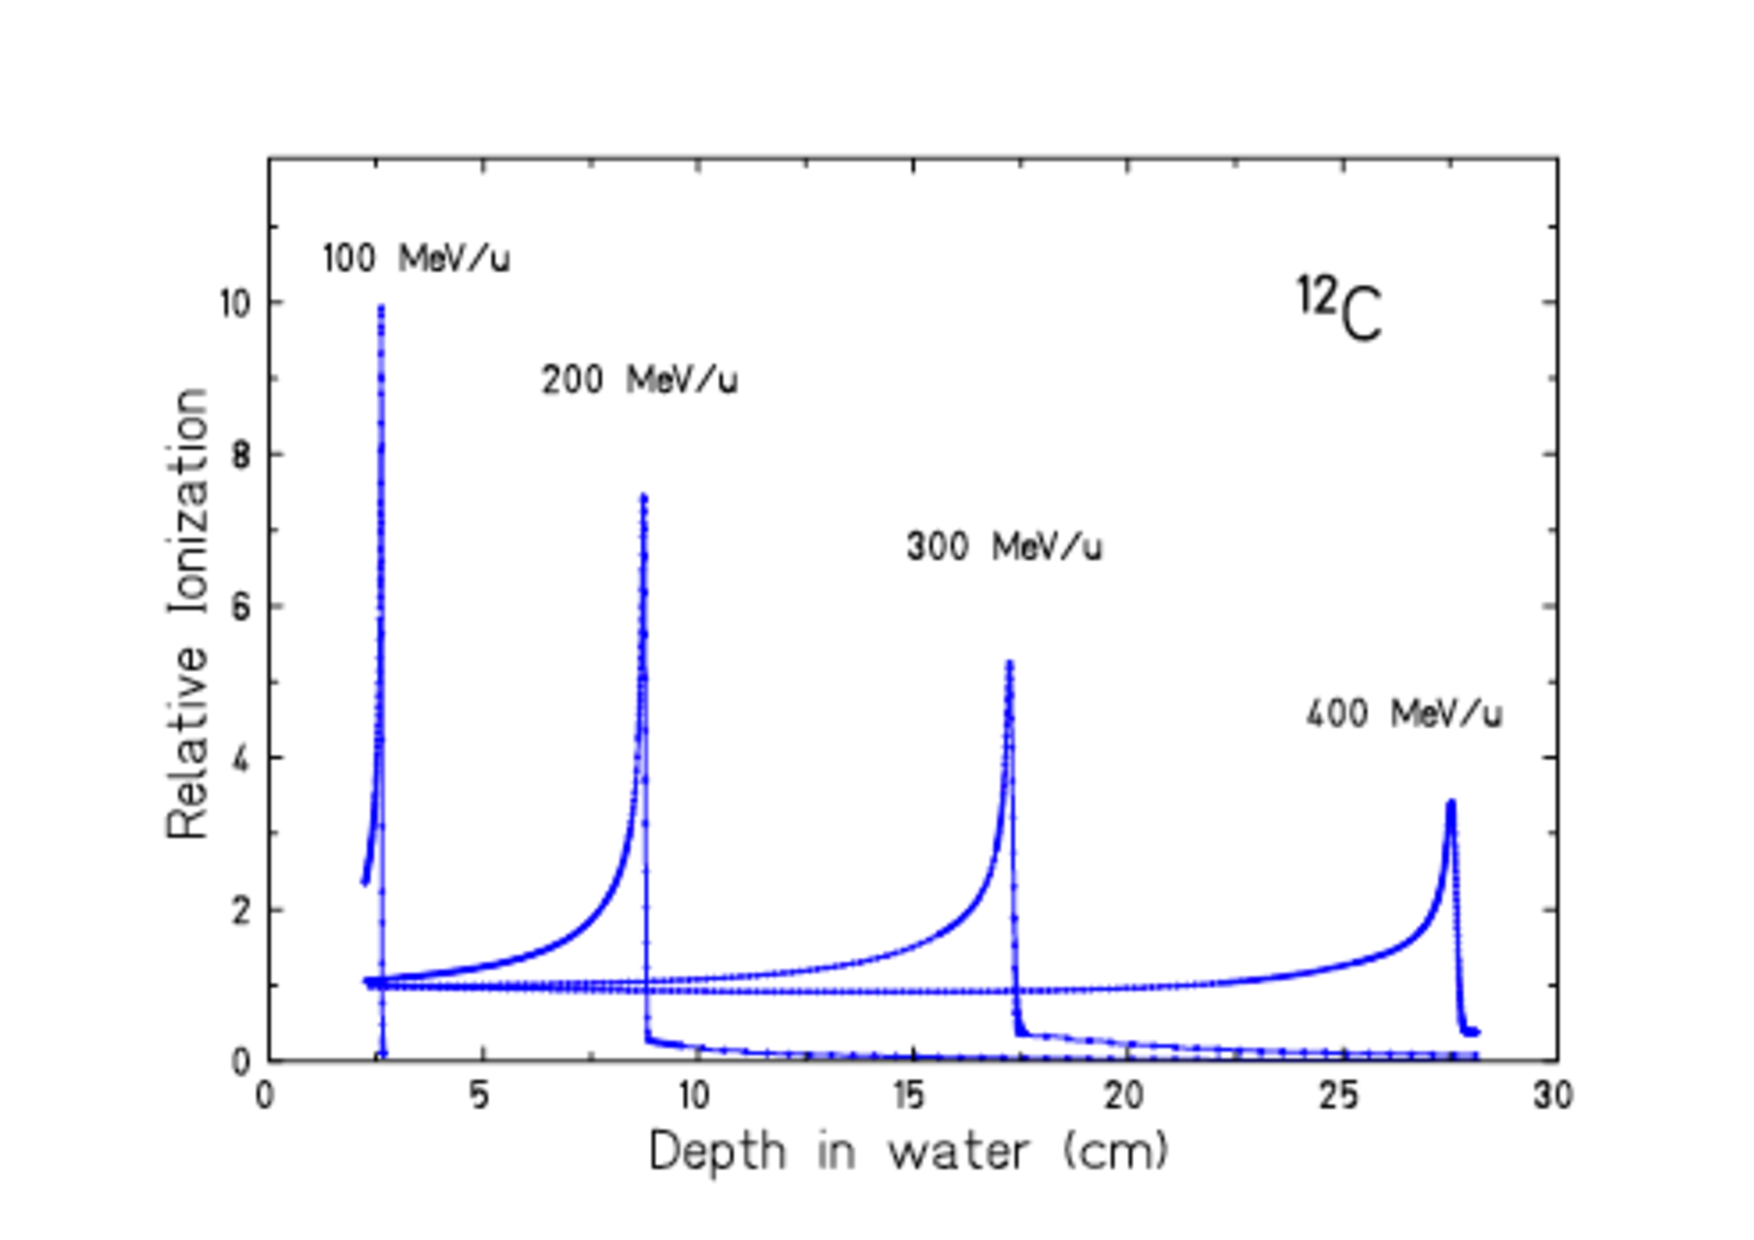
\includegraphics[width=0.92\linewidth]{03_GraphicFiles/chapter1_Introduction/tailBragg.pdf}	
\caption{Measured relative ionizations for car\-bon ion beams stopping in water (in~\cite{Schardt2008}).}
\label{chap1::fig::TailBragg}
\end{subfigure}
\caption{Effects of nuclear interactions on the primary beam and resulting dose distribution.}
\label{chap1::fig::NuclearInt}
\end{figure}

Further, interesting results about ion fragmentation in nuclear interactions can be found in~\cite{Matsufuji2003, Wroe2005, Haettner2006, Gunzert-Marx2008, Haettner2013}.

Detailed information about fragmentation can be retrieved via Monte Carlo simulations and used to evaluate the impact on the delivered dose. As an example, simulations published in~\parencite{Grassberger2011} of 160~MeV protons in water allowed to estimate the dose contributions given by primary particles (between 90\% and more than 99\% of the total depending on the range), with the remaining fraction of dose mainly connected to secondary protons and $\alpha$ particles: negligible dose is given by heavier fragments. A more intense dose contribution from heavier fragments is expected for carbon ion irradiation, but an accurate Monte Carlo simulation of these processes is still a challenge.

As mentioned, in addition to charged fragments, nuclear interactions also produce gammas, mainly originating from atomic de-excitation processes (prompt-gammas) or from the annihilation of positron emitted by beta-emitter fragments ($^{10}$C, $^{11}$C, $^{13}$N, $^{14}$O, $^{15}$O), and neutrons. All the secondary particles which can be absorbed by the target contribute to the total dispensed dose, while the others (with the exception of neutrons), escaping the target volume, can be exploited for non-invasive measurements of beam and target features. In particular, different techniques have been proposed and tested to measure secondary protons and gamma rays (both prompt-gammas and positron-annihilation gammas) with the aim of retrieving information about the ion range and obtain an online treatment verification. A detailed discussion about this topic will be given in section~\ref{chap1::subsec::secondaryRad}.

Focusing on neutrons, which are produced in large quantities and over a wide energy range, they cannot be exploited for primary ion range monitoring since they are not correlated with the ion path in matter~\parencite{Testa2010}. In any case, they must be modeled with care in order to evaluate the safety measures to be implemented in treatment centers~\parencite{Newhauser2002}, as well as the implications in the delivered dose and secondary cancer probability~\parencite{Newhauser2011}. The dose contribution caused by secondary neutrons strongly depends on the beam delivery system (see section~\ref{chap1::subsec::beamDelivery} for the description of the beam delivery systems), as demonstrated in~\cite{Gottschalk2006}. In particular, passive elements used for beam shaping have been identified as one of the main source of secondary neutrons contributing to the total delivered dose to the patient~\parencite{Yan2002}, so that in modern facilities deflecting elements are set after the passive modules in order to limit the neutron flux towards the target. It is interesting to notice that the amount of produced neutrons and resulting dose is compatible for protons and carbon ion irradiation, even if the neutron yield is higher for carbon ions: this is due to the different beam intensities used in clinics for the two species, with more than a factor 20 in favour of protons. Finally, if compared to photon standard radiotherapy, the neutron dose associated to ion beam therapy treatments results to be smaller, as demonstrated in recent studies~\parencite{Schneider2015}. 

More details about the physics of proton and, more generally, ion beam therapy, can be found in~\parencite{Lomax2009, Belkic2010, Schardt2010, Bichsel2013, Nupecc2014,  Newhauser2015, Durante2016}. In the following section, the attention is focused on the biological aspects of this cancer treatment modality.


\subsection{Biological effects of ion beam therapy}\label{chap1::subsec::bioEffects} 
In addition to the already presented physical differences between photon radiation therapy and ion beam therapy treatments, a fundamental aspect of the game lies in the biological effect of such radiations. In the following, the main biological implications of radiation therapy are summarized with the aim of highlighting the favorable contribution given by charged particles with respect to photons and, at the same time, discuss some controversial points~\parencite{Paganetti2013}.

Any kind of radiation interacting and deposing energy in human tissues causes ionizations which lead to cellular and molecular effects. The effectiveness of ionizing radiation in curing cancer is based on the consequences produced by these ionizations, which can affect the double-helical DNA macro-molecules inducing different kind of damages. In most of the cases, localized damages, also called strand breaks, can be repaired with cellular reparation processes. In case DNA breaks are in close proximity they can originate the so-called \glspl{dsb}, both with direct ionizations of indirect process (such as $\delta$-electron energy deposition). \figurename~\ref{chap1::fig::DNAdamages} shows a schematic view of the different kind of DNA damages induced by radiations, together with their effects in case of  successful or unsuccessful reparation mechanisms. \glspl{dsb} are generally harder to be repaired and lead to cellular dysfunction and loss of genetic material, resulting in cell death or in the loss of reproductive capacity. It appears clear from this simplified presentation that not only the total absorbed dose, but also the ionization event distribution plays a major role in the determination of the radiation effectiveness~\parencite{Belli1992}.        
The absorbed dose is defined in ~\cite{ICRU1980, ICRU1998} as 

\begin{equation}
\mathrm{D} = \frac{\mathrm{d}\overline{\epsilon}}{\mathrm{d}m}
\label{chap1::eq::AbsDoseDef}
\end{equation}

where $\mathrm{d}\overline{\epsilon}$ is the mean energy imparted by ionizing radiation to matter of mass $\mathrm{d}m$. To be precise, the imparted energy must also be defined: in the same ICRU reports we find that 

\begin{equation}
\epsilon = R_{\mathrm{in}} - R_{\mathrm{out}} + \sum{Q}
\label{chap1::eq::impEnergyDef}
\end{equation}

with $R_{\mathrm{in}}$ and $R_{\mathrm{out}}$ the sum of the energies of all ionizing particles entering or leaving the volume, respectively, $ \sum{Q}$ the sum of all changes of the rest mass energy of nuclei and elementary particles in any nuclear transformations occurred in the volume due to the ionizing radiation.
As mentioned, for the same absorbed dose, the ability of killing tumor cells is linked to the nature of the delivered radiations via the ionization event distribution. It is useful here to introduce the concept of \gls{let} \myMarginnote{Linear \\ Energy \\ Transfer}, defined as the amount of energy deposited by a particle per track unit, directly related to the number of ionization per unit distance. In general, photons, x-rays and $\gamma$-rays are referred to as low-\gls{let} radiation, while the larger stopping power of protons and ions make them a high-\gls{let} kind of radiation. For low-\gls{let} radiation, the distribution of the caused lesions is approximately random, while it is more closely related to the particle track for high-\gls{let} primaries~\parencite{Lobrich1996} causing a clustering effect in radiation damage which has been verified to be effective for cell killing\parencite{Holley1996, Rydberg1996}. This is due to the nature of interactions of photons and ions in matter, already detailed in the previous section. 
Photons transfer energy to the cells by photo-electric of Compton interactions, with rather low cross-sections which determine a small number of ionization events per incident photon within the cell volume. Many photons are then required to depose the prescribed dose, and given the random spatial distribution of the photons in the irradiating beam, the resulting ionization distribution is almost homogeneous. The physical interactions of ions determine a completely different distribution of the deposited energy, localized along the ion path. The dose imparted in the radial direction is governed by freed electrons ($\delta$ or Auger electrons), emitted in ion-atom interactions, which are scattered by the medium atoms (electrons and nucleus) and cause secondary ionizations. The cross-section of these ionizations exhibits a maximum at about 100~eV, corresponding to a mean free path of a few nm. Given the DNA molecule size, this effect leads to a high probability of creating \glspl{dsb} or correlated single-strand breaks. %Thus, the lesion complexity increases with \gls{let}, and the strand breaks more concentrated in space are hardly repaired by the involved cells. 
Cell survival studies~\parencite{Tobias1982, Blakely1984} verified these theoretical considerations showing that heavy charged particles have an increased biological effectiveness compared to x-rays. These data are generally analyzed with a parametrization of the cell survival curve through a \gls{lq} model~\parencite{Hall2012}

\begin{equation}
S(D) = \mathrm{exp}(-\alpha D - \beta D^{2})
\label{chap1::eq::survivalPar}
\end{equation}
where S is the survival fraction, D is the absorbed dose and $\alpha$ and $\beta$ are parameters which are experimentally determined, or obtained via radio-biological models (see section~\ref{chap1::subsec::treatmentPlan}). The $\alpha/\beta$ ratio is linked to the radio-sensitivity of cells: the smaller it is, the larger the DNA repair capability will be. This is the rationale for fractionation in radiation therapy. In effect, the total dose planned for the treatment of malignant cells is delivered in fractions along several days, because split doses have the advantage to spare normal tissues, with low $\alpha/\beta$ ratio, more than tumors, showing higher $\alpha/\beta$ ratio. 

\begin{figure}
\begin{subfigure}[t]{.4\textwidth}
\centering
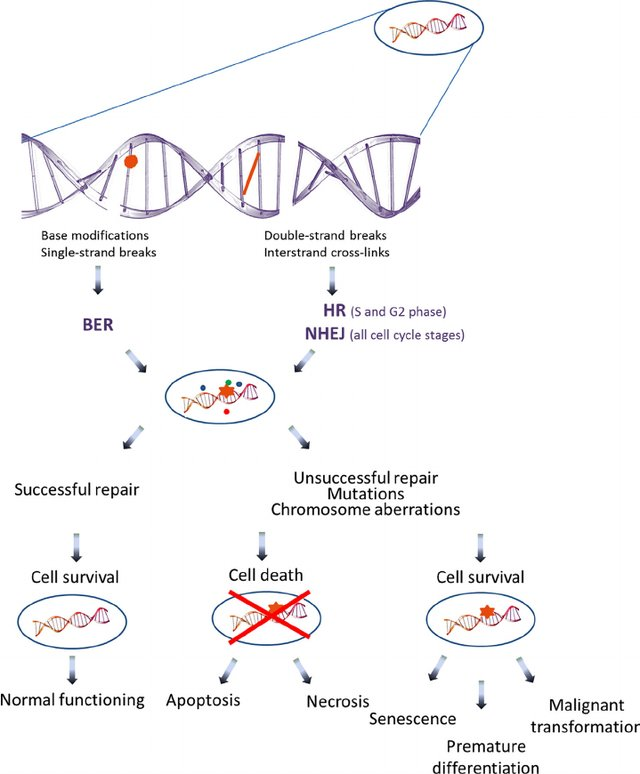
\includegraphics[width=0.99\linewidth]{03_GraphicFiles/chapter1_Introduction/DNAdamage.jpg}
\caption{Schematic representation of DNA damages caused by radiations. In~\cite{Arena2014}.}
\label{chap1::fig::DNAdamages}
\end{subfigure}
\begin{subfigure}[t]{.58\textwidth}
\centering
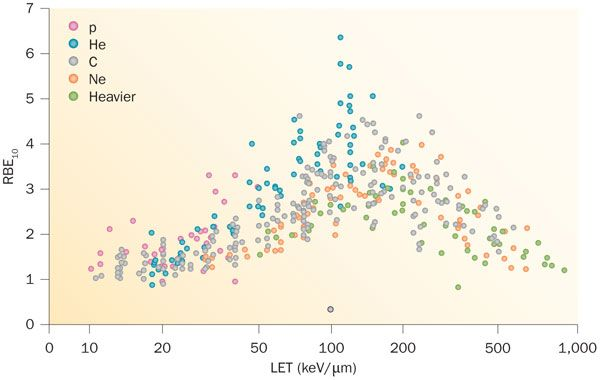
\includegraphics[width=0.99\linewidth]{03_GraphicFiles/chapter1_Introduction/rbeLET.jpg}	
\caption{\gls{rbe} dependence on \gls{let} for different particle species. \gls{rbe} is calculated at 10\% survival, \gls{let} values are given is keV/\charmum  ~in water. Different ions are represented in different colors. Data points are extracted from the \gls{pide} database. In~\cite{Durante2016}.}
\label{chap1::fig::rbelet}
\end{subfigure}
\caption{Ionizing radiations cause DNA damages in tissues, which are the basis for tumor radiation therapy. On the left side, the scheme presents the possible kind of damages induced by radiations on the cell DNA. The radiation effectiveness in killing cells is then related to the distribution of ionization events, which is all the more dense for high-\gls{let} primaries at low energies. The \gls{rbe} is then enhanced for this kind of radiation. On the right side, the \gls{rbe} is related to the \gls{let} for different ion species.}
\label{chap1::fig::NuclearInt}
\end{figure}
     
Given the complex scenario presented till here, it is clear that the physical absorbed dose is not sufficient to describe the effect of the delivered radiation treatment, and weighting factors based on radiation protection data have been introduced to account for both the biological properties of ions and the response of different tissues. However, \myMarginnote{Relative \\ Biological \\ Effectiveness} in order to transfer the experience from photon data to ion irradiation and to create a common evaluation parameter, the more powerful and versatile concept of \gls{rbe} has been introduced. The \gls{rbe} is defined as the ratio between the photon and ion doses necessary to produce the same biological effect (isoeffective dose):

\begin{equation}
\left. \mathrm{RBE} = \frac{D_{\mathrm{photon}}}{D_{\mathrm{ion}}}\right|_{iso}
\label{chap1::eq::rbeDef}
\end{equation}

where $D_{\mathrm{photon}}$ and $D_{\mathrm{ion}}$ are the absorbed dose for photon and ion irradiation. Notwithstanding the apparently simple definition, \gls{rbe} results to be a very complex quantity, but for the moment the only one really used in clinics. It depends on several physical and biological parameters, such as \gls{let}, dose, dose rate, fractionation scheme, particle type, target biological features (radiosensitivity, oxygen concentration, etc.)~\parencite{Durante2009}. As a result, the \gls{rbe} value changes along the primary ion path in matter, and is very difficult to be accurately predicted at the treatment planning stage. As an examples, the dependence on \gls{let} is shown in \figurename~\ref{chap1::fig::rbelet}.  Although an accurate prediction is difficult to be obtained, the overall evolution of the \gls{rbe} as a function of \gls{let} demonstrate a further advantageous feature of ions with respect to photons. From very low \gls{let} to approximately 100-200~keV/\charmum ~, the \gls{rbe} increases: an overkilling effect determines then a drop at very high \gls{let} values. Thus, \gls{rbe} is higher for low energetic high-\gls{let} particles, which cause larger ionization density as their velocity decrease. This effect means that in the Bragg peak region the biological effectiveness of such radiations is more pronounced with respect to the plateau entrance area, where healthy tissues are spared. The \gls{rbe} enhancement for increasing \gls{let} is at present neglected in proton therapy, and a constant value of 1.1 is implemented in the clinical routine. This point is deeply discussed in the last years, and many simulation results and models have been produced to verify or propose modification to this usage~\parencite{Giantsoudi2013, Sethi2014, Guan2015, Jones2015, McNamara2015, Giovannini2016}. Anyway,  it is verified that a significant increase in \gls{rbe} with respect to photons can only be achieved with heavier ions, as also shown by the experimental data reported in \figurename~\ref{chap1::fig::rbelet}. For this reason, clinical trials have been conducted at the Lawrence Berkeley Laboratory starting from 1975 on different ion species such as He, Ne, N, O, C, Si, Ar~\parencite{Castro1995}. Very heavy ions have the advantage of providing very-high \gls{let} (and so \gls{rbe}) in the Bragg peak region, useful to overcome cell killing capability limitation due, for example, to cell oxygenation effects (discussed in the following)~\parencite{Blakely1984}. On the other side, heavy ions also show very high \gls{let} in the entrance region, which is not desirable. These results led to the implementation of carbon ion therapy, together with proton therapy, as a good comprise between radio-biological enhanced effectiveness in the target region and limited \gls{let} in the plateau. 
As outlined in previous lines, a further parameters to account for in the evaluation of the biological effects of radiations is the cell oxygen status \myMarginnote{Oxygen Enhancement Ratio}. If compared to healthy tissues, tumor masses can grow in size producing low quality cells, which are generally concentrated in the tumor core and show lower oxygen levels. Even if the reason is not completely explained, hypoxic conditions cause an increased cell radio-resistance, probably linked to the reduction of indirect DNA damages induced by radicals. This effect is quantified via the \gls{oer}, 

\begin{equation}
\mathrm{OER} = \frac{D_{\mathrm{hypoxic}}}{D_{\mathrm{aerobic}}}
\label{chap1::eq::oer}
\end{equation}

with $D_{\mathrm{hypoxic}}$ and $D_{\mathrm{aerobic}}$ the absorbed dose for normal and reduced oxygen level resulting in the same clinical effect. Its value is about 3 for conventional radiation~\parencite{Schardt2010}, while it is reduced for ion irradiation due to the increased \gls{rbe}, making then fundamental for curing tumors with hypoxic regions.

Only some of the biological aspects have been cited here, and all their clinical implications should be ideally taken into account for an accurate treatment planning. This is the reason why some of the points discussed here will be further addressed in section~\ref{chap1::subsec::treatmentPlan}. 

\subsection{Accelerators and beam delivery}\label{chap1::subsec::beamDelivery}

The goal of ion beam therapy is to treat deep-seated tumors with a conform dose distribution. Different ion species, hadrons and charged particles in general have been and are under study for the clinical application (neutrons, charged pions, antiprotons, helium ions - i.e. alpha particles -, heavier ions like lithium, oxygen, up to silicon ions), but only two are at present implemented for the patient treatments: protons and fully stripped carbon ions~\parencite{Degiovanni2015}. The ability of treating any kind of tumor at any depth in human body relies on the possibility of providing the employed particles enough energy to obtain a range of about 25~cm in soft tissues. The ions employed in treatment must be then accelerated to about 60-70\% of the speed of light ($\beta$ = 0.6-0.7, see~\cite{Durante2016}) via different acceleration techniques and machines. This translates into maximum energy values of the order of 200-250~MeV and 4500~MeV (i.e. 375~MeV/u) for protons and carbon ions, respectively~\parencite{Braccini2010}. In order to achieve the desired ion energy,  sizable accelerators are needed and different solutions have been explored; at present, cyclotrons and synchrotrons  are clinically implemented and available on the market. In the following, after a brief historical introduction, we sketch the main characteristics of the accelerators used in clinics, and we highlight the main features which are reflected in the treatment delivery. In addition to this, the beam delivery systems are described. Moreover, an overview of the main directions followed for the future acceleration and beam delivery techniques upgrade is provided. 

\subsubsection{Accelerators for ion beam therapy}\label{chap1::subsubsec::accelerators}
The way towards the possible application of ion beams in therapy \myMarginnote{Cyclotrons} (proposed only later by Wilson - see~\cite{Wilson1946}) was opened by the invention of the cyclotron by Ernest Orlando Lawrence in 1929~\parencite{Lawrence1932}, which added a magnetic field to the recently proposed linear accelerator~\parencite{Wideroe1928}. A cyclotron is composed of two hollow electrodes with a frequency-alternating voltage applied between them, which accelerates the charged particles at each revolution. The circular trajectory is obtained thanks to a fixed vertical magnetic field. A scheme of the main components of a cyclotron is sketched in \figurename~\ref{chap1::fig::cyclotron}.

\begin{figure}[!htbp]
\centering
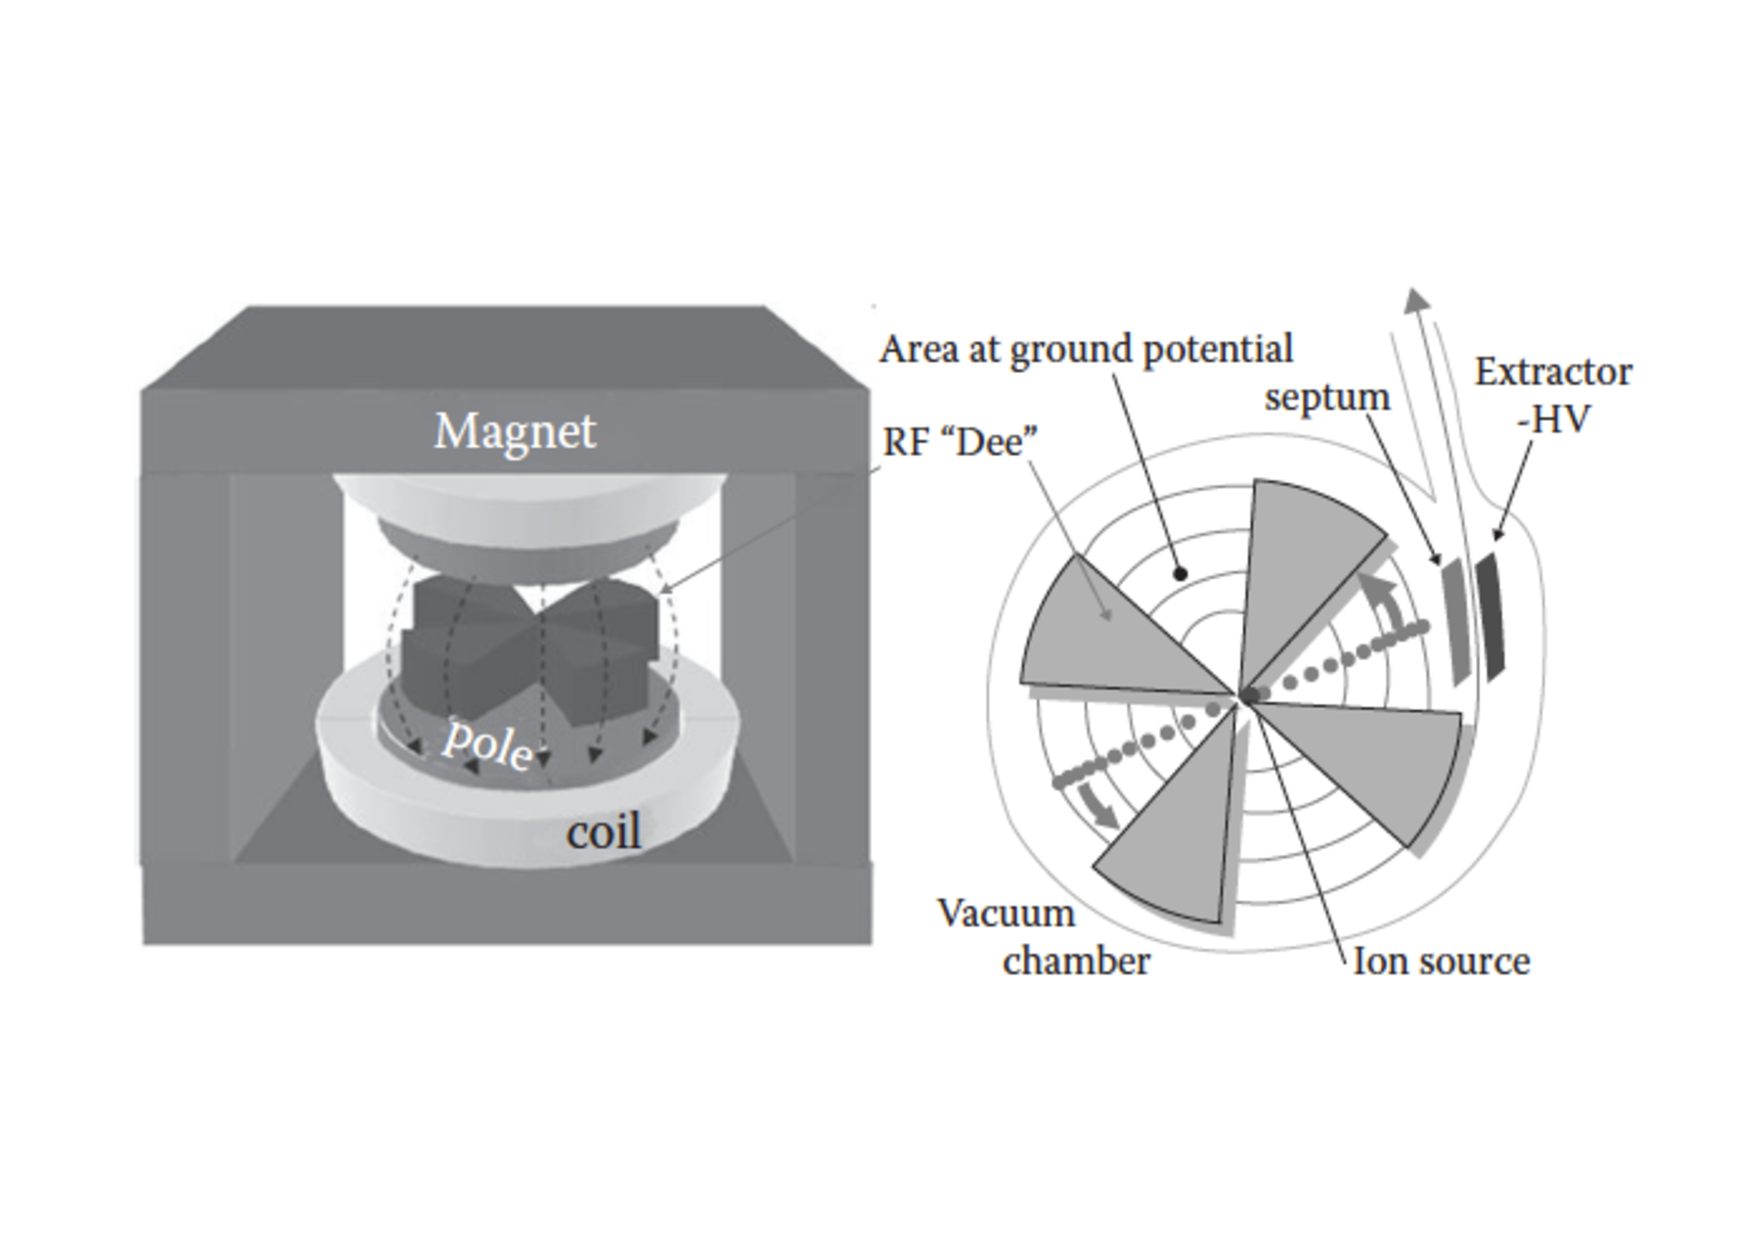
\includegraphics[width=0.7\textwidth]{03_GraphicFiles/chapter1_Introduction/cyclotron.pdf}
\caption{Schematic view of the main components of a cyclotron accelerator. On the left side the magnet is sketched together with the radio-frequency elements (\enquote{Dees}), which are also shown on the section depicted on the right side, with the ion source in the center. In~\cite{PaganettiBook2012}.}
\label{chap1::fig::cyclotron}
\end{figure} 

Nuclear physics saw a paramount development thanks to this invention, but also in the medical field the impact was remarkable. Already in 1935, Lawrence produced the first cyclotron-originated radionuclides, then used for radiotracing, diagnosis and treatment. The first cyclotron-based treatment was performed with fast neutrons (i.e. with kinetic energies between a few MeV and a few tens of MeV) in 1938, following a paper by Gordon Locher who underlined the therapeutic potentialities of neutrons~\parencite{Locher1936}; the neutrons were produced by bombarding a beryllium target with cyclotron-accelerated deuterons~\parencite{Stone1940}. The unfavorable depth-dose distribution of neutrons and the difficulties linked to their collimation finally led to abandon the neutron treatments in 1948~\parencite{Stone1948} and move towards proton-beam treatments in the 50's: neutrons were revised in 1965 by Catterall in London~\parencite{Catterall1971} and are still used today in \gls{bnct} techniques~\parencite{Barth2005, Nedunchezhian2016}. As already mentioned in section~\ref{chap1::sec::ionBeamTher}, the first proton therapy treatment was conducted by Cornelius Tobias,  and John Lawrence with the Lawrence cyclotron in 1954~\parencite{Tobias1955, Tobias1958}. Between 1954 and 1974, more than 100 patients were treated in Berkeley with cyclotron-accelerated protons. In parallel, in 1957 the first tumor was irradiated with protons at the Uppsala cyclotron in Sweden~\parencite{Larsson1962}, and an intensive proton therapy program, leaded by Robert Wilson, was started in Harvard with a new-built cyclotron~\parencite{Wilson2004}. Following these first experiences, new physics laboratories decided to set up proton beams for therapy (USSR, Japan, Switzerland), until the creation of the first hospital-based center, built at the Clatterbridge Oncology Center in the United Kingdom, which started operating in 1989 with a 62.5~MeV cyclotron. This historical overview shows how the cyclotron technology has soon spread all over the world, not only in research centers, but also for therapy purpose. The present cyclotron machines, which are now commercially available by different providers,  still rely on the same accelerating principle as the first Lawrence system, but the technology has greatly advanced.  In particular, the vertical magnetic fields in charge of bending the particles on a spiral trajectory has been improved, giving the beam the desired transverse compactness. Moreover, the beam extraction efficiency has been improved, and multiple extractions are now possible to supply different transport lines.
Moreover, synchrocyclotrons are a solution compatible with hadrontherapy applications. Based on the cyclotron accelerating principle, a synchrocyclotron presents a variable frequency for the alternating voltage which is used to compensate for relativistic effects when the accelerated ions approach the speed of light. Such a solution has the advantage of allowing for the creation of more compact systems with high magnetic fields, and is at present exploited for commercial accelerators by the main providers.  
In addition to cyclotrons and synchrocyclotrons, other accelerating machines \myMarginnote{Synchrotrons} initially developed for fundamental research have been translated to medical applications and are nowadays knowing a large diffusion: the synchrotrons. While the cyclotron present a fixed-value magnetic field, so that the radius of the beam trajectory increases during the acceleration process, in the synchrotron the trajectory radius is kept constant thanks to the variation of the bending magnetic field. The boost is provided by radio-frequency cavities, based on the same principle as the one composing linear accelerators: the radio-frequency increases to follow the particle revolution speed, and this acceleration principle allows to overcome the cyclotron energy limitation, as well as to obtain beam at different energies by tuning the extraction process. The invention is based on the independent ideas of Vladimir Veksler~\parencite{Veksler1944} and Edwin McMillan~\parencite{McMillan1945}: the latter both coined the name of the machine in its letter, and constructed the first electron synchrotron in 1945 in Berkeley. Some years later, the first proton synchrotron was designed in 1952 by Sir Marcus Oliphant, which already published a preliminary sketch of the machine in 1943~\parencite{Oliphant1943}. As for the cyclotron case, several years have been required to see the construction of the first hospital-based hadrontherapy facility using a synchrotron. The first center was built at Loma Linda University in California, were a 7-m-diameter synchrotron constructed by Fermilab was installed and started treating patients in 1990. The center has been a pioneer in the field also for the presence of three 10-m-diameter rotating gantries.  
After the clinical studies performed at the University of Tsukuba, in Japan, between 1983 and 2000, with the treatment of about 700 patients with synchrotron proton beams, a second hospital-based center was built and equipped with an Hitachi synchrotron and two rotating gantries. 
Since the first use of synchrotrons for treatment purpose, several improvements have been achieved in the accelerator technology to better adapt its features to the hadrontherapy needs. In particular, the beam size can be now reduced with strong focusing optics, and the beam energy can be varied on a single spill basis, in contrast to the first machines for which 1-2~s were needed to modify the spill energy.   
At present, all the hadrontherapy facilities in operation are based on circular accelerators (cyclotrons and synchrotrons): proton beams are produced with both the solutions, while only synchrotron-produced carbon-ion beams are used. In \figurename~\ref{chap1::fig::acceleratorSize} the size of different accelerators design is compared (CABOTO is still at the design stage, the \gls{iba} superconducting synchrotron is under installation in France, while \gls{hit}, \gls{cnao} and the SIEMENS accelerator are at present in operation).

\begin{figure}[!htbp]
\centering
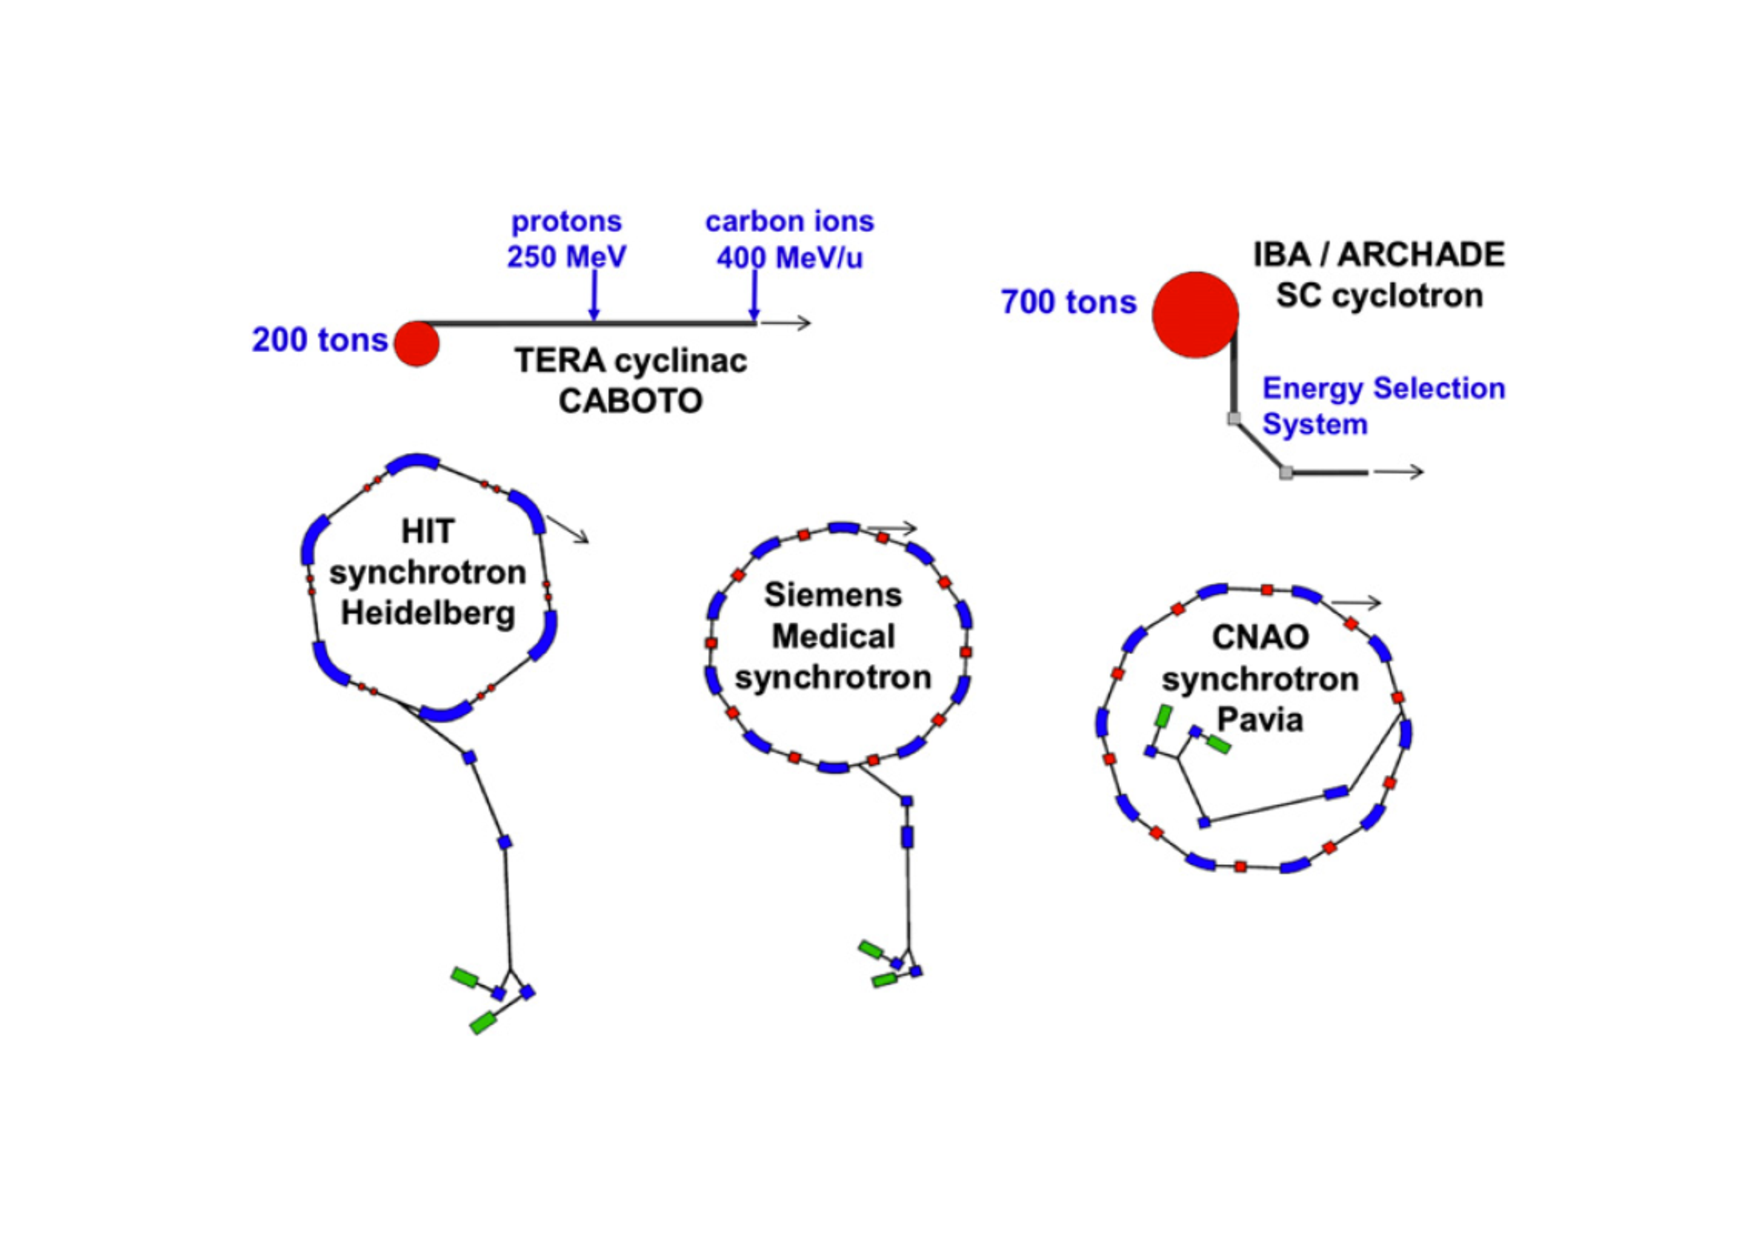
\includegraphics[width=0.7\textwidth]{03_GraphicFiles/chapter1_Introduction/acceleratorSize.pdf}
\caption{Comparison of the size of various ion accelerators for hadrontherapy. CABOTO is a cyclinac studied by the TERA Foundation; the superconducting cyclotron, designed by \gls{iba}, is under installation in Caen, France, within the ARCHADE project; \gls{hit} and \gls{cnao} are in operation in Heidelberg, Germany and Pavia, Italy, respectively; the SIEMENS synchrotron is installed in Marburg and Shangai. In~\cite{Amaldi2010}.}
\label{chap1::fig::acceleratorSize}
\end{figure} 

In the last years, novel approaches has been proposed \myMarginnote{Novel acceleration approaches} to improve the present accelerators and beam features, mainly for what concerns the beam quality and the machine size and cost. It is worth to mention the \gls{ffag} accelerator, which combines the fixed magnetic field and variable radio-frequency with separated sector magnets~\parencite{Sheehy2016}. This approach allows for the production of higher intensity beams with respect to synchrocyclotrons, and for the variation of the extracted beam energy at high repetition rate. Some design have been proposed for hadrontherapy applications in the last decade~\parencite{Antoine2009, Peach2010}, but the present machine size still limit its spread in treatment centers. 
Furthermore, linear acceleration approaches has been proposed since 1991 in both \enquote{all-linac}~\parencite{Lennox1991, Hamm1991} and \enquote{cyclinac}~\parencite{Amaldi2009b} solutions. In addition to the compactness, the main advantage of linacs is the possibility to continuously vary the output beam energy on a pulse to pulse basis; in addition to this, there is neither the need for complex injection or extraction systems, such the ones used in synchrotrons, nor the need of an energy passive modulation technique as the one used in cyclotrons (see section~\ref{chap1::subsubsec::BeamDel}). An extended description of linear accelerators for hadrontherapy is given in~\cite{Amaldi2009a}. Following the first successful prototypes tested by the TERA Foundation and the Italian \gls{infn} in the last twenty years~\parencite{Amaldi2004, Ronsivalle2011}, the \gls{cern} spin-off company \gls{adam} is proposing a commercial solution called \gls{light}. A further solution can be given by the \gls{dwa}~\parencite{Caporaso2009}, where the acceleration tube is made of High Gradient Insulator disks alternated with conducting elements. A laser pulse is used to activate the switching units connected to these conducting modules. Very interesting thanks to a reduced size, this acceleration scheme still suffers beam focusing issues; moreover, it presents very short pulses which force a very precise selection of the number of ion per pulses at the source level. Finally, the electric field needed for reducing the machine size till 2-2.5~m is of the order of 100~MV/m; this challenging value has not been achieved yet, even if a prototype is under study at the \gls{llnl}, with promising results~\parencite{Hettler2013, Zografos2013}. Another attractive technique is the so-called \enquote{laser driven} acceleration, based on the use of short and powerful laser pulses irradiating a thin target, with the generation of a plasma field~\parencite{Tajima2009}. The electrons emerging form this plasma are able to induce a strong electric field which accelerates the protons (or ions). Again, this solution would allow for the creation of very compact systems, with relatively simple and light beam optics, but some issues are still under study to be solved; in particular, the accelerated beam has an almost continuous energy spectrum which forces to implement energy modulation solutions to be adapted to treatment purposes. 

\subsubsection{Beam time structure}\label{chap1::subsubsection::beamTimeStruct}

A particle beam can be described by a set of quantifying parameters which relates to single particle properties or to a collection of particles. In addition to the beam energy (which should be defined as an energy spectrum), beam current (which describes the beam intensity as the flux of particles per time unit) and transverse size, it is worth to describe in details what is defined as time structure. A basic distinction is made between continuous beams and bunched beams. Whenever particles are accelerated by means of radio-frequency varying fields, the accelerating machine output is a bunched beam, composed of bunches with fixed time length. Concerning the acceleration systems employed to produce clinical beams, synchrotron and cyclotrons (or synchro-cyclotrons) present strongly different time structures. In order to give an overall description of the typical time features of synchrotron- and cyclotron-produced beams, it is possible to distinguish between micro- and macro-structure. The macro-structure describes cycles of several radio-frequency periods, while the micro-structure gives the details of the particle time distribution within the same radio-frequency period. By comparing the two cited kinds of accelerators, it is possible to approximate the cyclotron-produced beams as continuous, with a macro-structure characterized by sub-millisecond periods (depending on the specific machine). In contrast, synchrotrons produce pulses which are separated in periods of several seconds, so that during the irradiation the active beam time is limited. Each accelerator pulse (for both cyclotrons and synchrotrons), corresponding to one \gls{rf} period, contains several micro-bunches, creating the micro-structure. For cyclotrons, micro-bunches duration is in the ns scale, while a synchrotron micro-bunch can last several tens of ns. The period separating micro-bunches varies in the range of tenths of ns for cyclotrons till hundreds of ns for synchrotron beams. 

Table~\ref{chap1::tab::beamTime} shows the orders of magnitude for the beam time structure for some particle accelerators used in the clinical routine. The differences between synchrotrons, cyclotrons and synchro-cyclotrons are evident. In addition, the beam typical intensity is also reported.

\begin{table}[!htbp]
\centering
\caption{Orders of magnitude of main time structure parameters for some accelerators used in clinics.}
\label{chap1::tab::beamTime}
\begin{tabular}{P{2cm} P{2cm}  P{1cm} | P{1cm} P{2cm} P{2cm} P{2cm}}
\toprule
\rowcolor{myColorMainA!20} 
 	& &  \multicolumn{2}{c}{\textbf{Synchrotron} }& \textbf{Cyclotron C230 \gls{iba}} & \textbf{Cyclotron Varian} & \textbf{Synchro-cyclotron S2C2 \gls{iba}}\\
& & \underline{$^{12}$C} & \multicolumn{4}{c}{\underline{Protons}} \\
\midrule
\multicolumn{2}{l}{\textbf{Typical intensity (ions/s)}} & 10$^7$ & 10$^9$ & 10$^{10}$ & 10$^8$ - 10$^{10}$& $\sim$10$^{10}$ \\
\midrule
\textbf{Macrostruct.} & Period (s) & \multicolumn{2}{c}{1-10} & \multicolumn{2}{c}{/} & 10$^{-3}$ \\
\midrule
 & Bunch width & \multicolumn{2}{c}{20-50} & 1-2 & 0.5 & 8 \\
\textbf{Microstruct.}  &  Period (ns) & \multicolumn{2}{c}{100-200} & 10 & 14 & 16\\
 & Ions/bunch & \multicolumn{2}{c}{2-5} & 200 & 2-200 & 4000 \\
\bottomrule
\end{tabular}
\end{table}      

An accurate knowledge of the beam time structure is of utmost importance for the optimization of the interface to the beam delivery systems (see section~\ref{chap1::subsubsec::BeamDel}), for the treatment planning, as well as for treatment monitoring purpose. The design of detectors able to exploit the emission of secondary particles to retrieve beam range and dose information must account for the beam time structure in order to evaluate the best solution to deal with signal background, counting rate and read-out channel occupancy. This topic will be further discussed in section~\ref{chap1::subsec::uncertainty} where the sources of uncertainties affecting ion beam therapy treatment are described and the detection monitoring solutions are presented. In particular, for the specific case of \gls{pg} detection (one of the main topic of this thesis work), a complete overview is given in chapter~\ref{chap::2}. 

\subsubsection{Beam delivery systems}\label{chap1::subsubsec::BeamDel}

Once accelerated, the high-energetic ions must be delivered to the patient in order to be conform to the treatment specification, focusing the provided dose on the \gls{ptv}. As described and detailed in section~\ref{chap1::subsec::Physics}, the beam range can be varied by modulating the primary particle energy with the aim of covering the whole tumor volume. The Bragg curve obtained with a monoenergetic beam is called \enquote{pristine Bragg curve}, and can be used to irradiate a section of the target volume at a given depth. The superposition of several pristine Bragg curve is necessary to deliver the prescribed dose to the tumor, which has been previously modeled in three dimensions. In particular, the beam energy spectrum has to be spread in order to increase the axial dimension of the peak region, in the so-called \gls{sobp}. At the same time, the beam fluence must be adapted to avoid over-irradiation of the entrance region. An example of \gls{sobp} is given in \figurename~\ref{chap1::fig::pristine_sobp}.

\begin{figure}[!htbp]
\centering
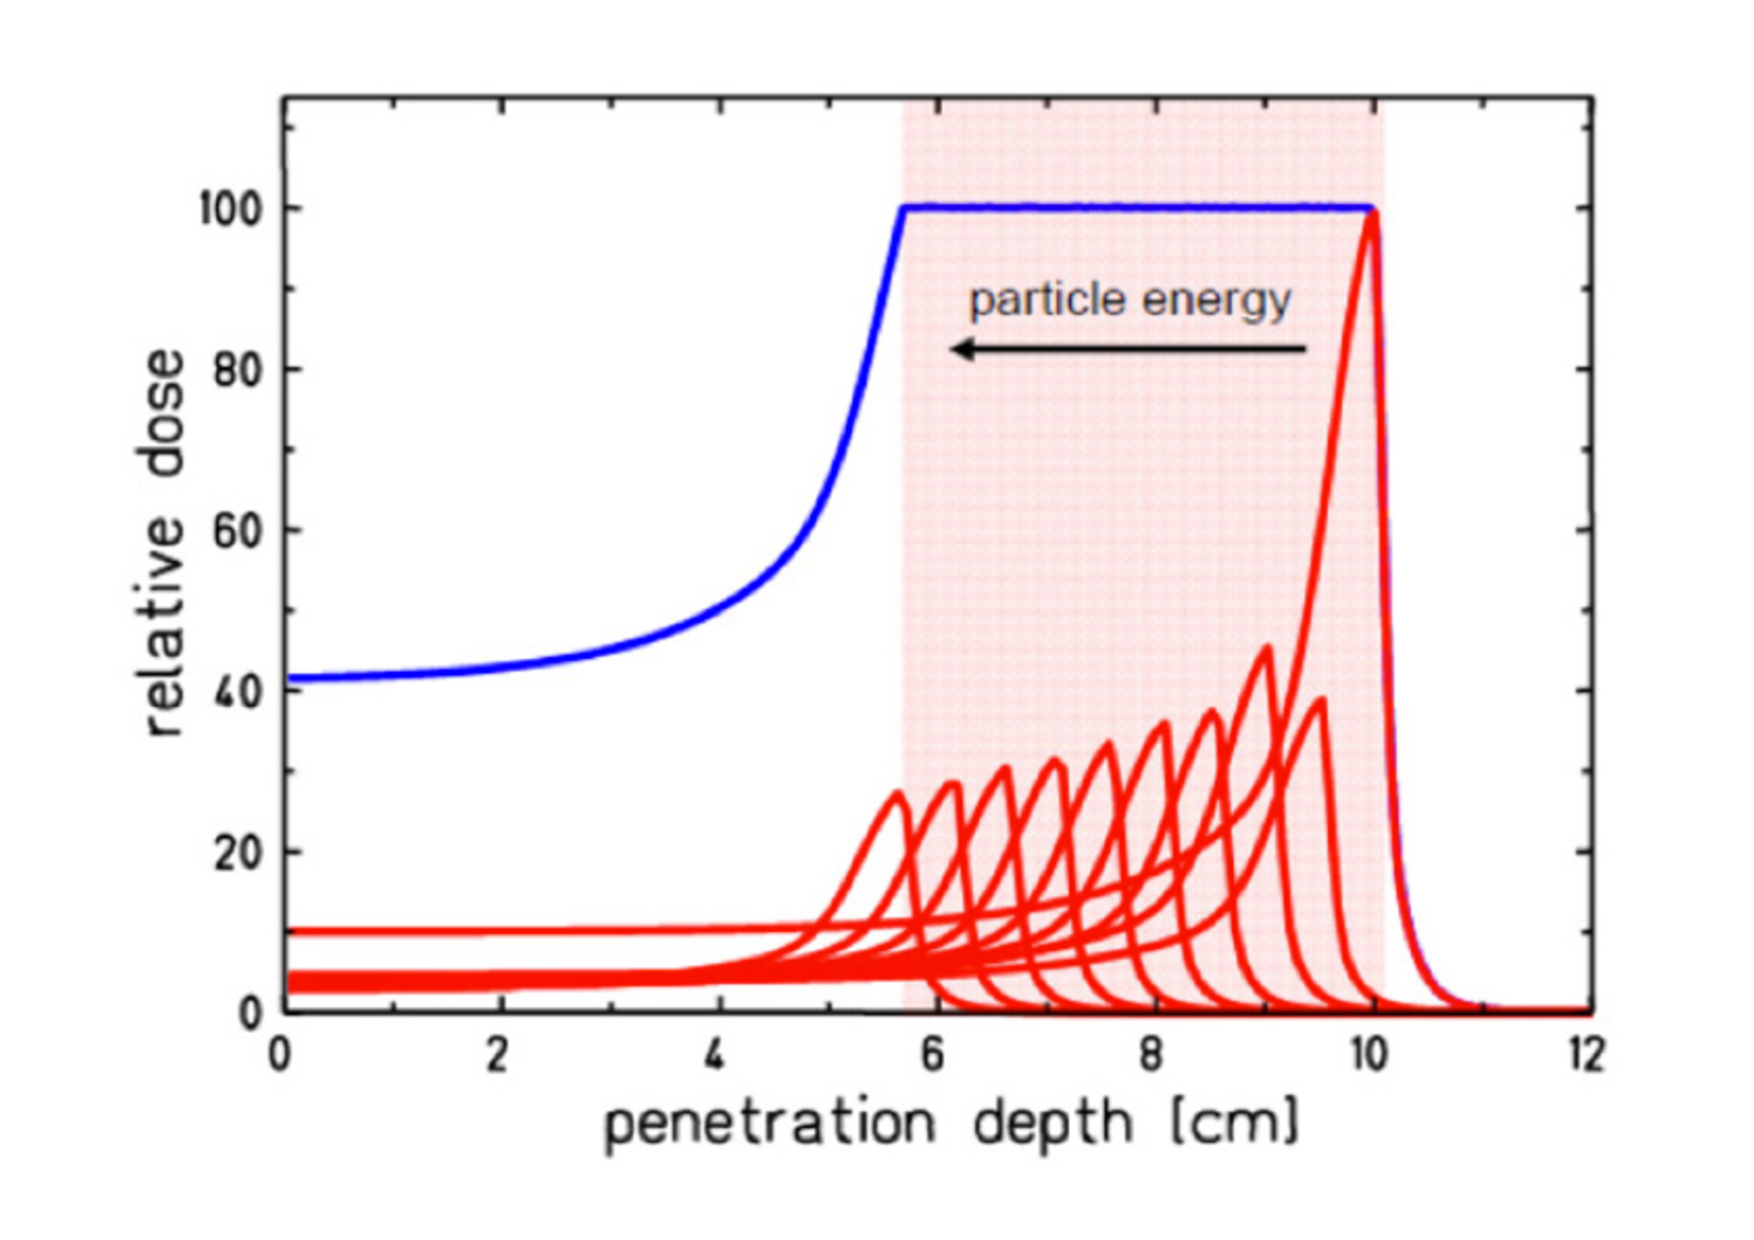
\includegraphics[width=0.7\textwidth]{03_GraphicFiles/chapter1_Introduction/pristine_sobp.pdf}
\caption{Example of \gls{sobp}. The target regione is highlighted and the discrete pristine peaks composing the \gls{sobp} are sketched in red. In~\cite{Durante2016}.}
\label{chap1::fig::pristine_sobp}
\end{figure} 

All these tasks are in charge of the beam delivery system, which must be optimized to interface with the accelerator and to the patient by transporting the beam to the treatment area and adjusting its features to obtain the desired dose distribution. 
The delivery systems implemented in clinics are based on two main strategies: passive beam modulation and active scanning. For an extensive presentation of this topic, refer to~\cite{Gottschalk2008}. The chosen technique must be chosen according to the accelerator machine: it is important to recall that cyclotrons provide fixed energy beams with pulses separated by about 10-20~ns, while in a conventional synchrotron the energy can be varied cycle by cycle, with short pulses generally separated by 1-2~s dead-time (see section~\ref{chap1::subsubsection::beamTimeStruct}). 

The passive beam delivery approach \myMarginnote{Passive beam shaping} generally applies to cyclotron produced beams, and its principle is sketched in \figurename\ref{chap1::fig::passiveDelivery}. The beam extracted from the accelerator is fixed in size and energy, and is first broadened by scattring devices. Afterwards, a range modulator (generally a rotating wheel) is used to spread out the monoenergetic Bragg peak with the aim of covering the whole target volume. The wheel periodically inserts material of varying thickness into the beam line, resulting in a range modulation at the desired frequency. The obtained \gls{sobp} can be shifted as a whole thanks to the addition of range shifters of fixed thickness. After the energy (range) adaptation, the beam is shaped according to the \gls{ptv} definition with collimators (often multi-leaf) and compensators, which are specific to each patient.  

\begin{figure}[!htbp]
\centering
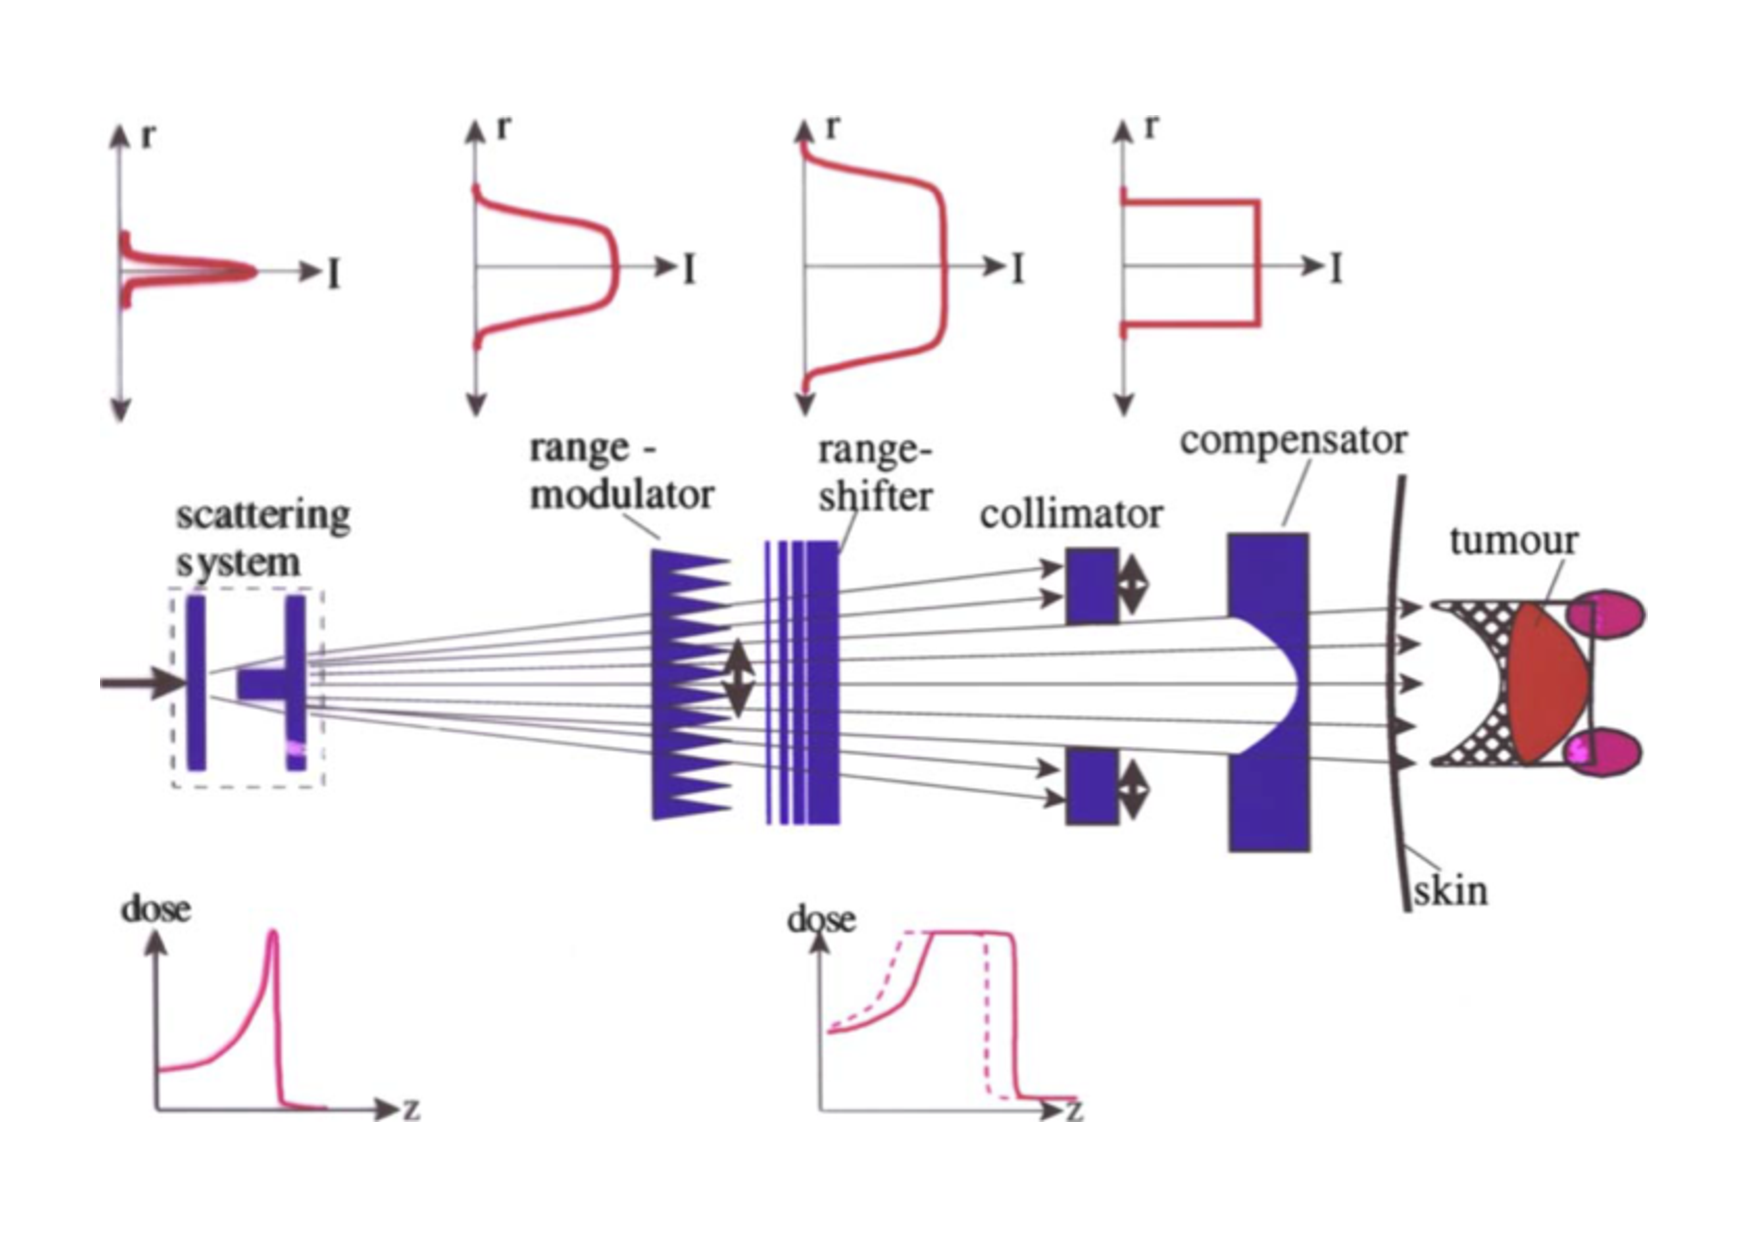
\includegraphics[width=0.7\textwidth]{03_GraphicFiles/chapter1_Introduction/passiveDelivery.pdf}
\caption{Schematic view of a fully passive beam delivery system. In~\cite{Schardt2010}.}
\label{chap1::fig::passiveDelivery}
\end{figure} 

The passive beam delivery technique presents two main disadvantages with respect to the active delivery described in the following. First, the structure of the created \gls{sobp} is fixed so and the depth-dose can only be tailored to the distal end of the target volume and not to the proximal end, given the fact that the \gls{sobp} can onlt be shifted towards the entrance region. This feature automatically leads to a considerable dose is given to normal tissues outside the target volume, in particular in the proximal part. Second, the amount of material inserted in the beam line causes nuclear interactions which lead to the creation of secondary high-\gls{let} fragments (mainly neutrons), affecting the dose delivered to the entrance region.

When the beam is produced with a synchrotron, \myMarginnote{Active beam scanning} the possibility to switch the energy from pulse to pulse makes feasible an active target scanning and beam range adaptation. The active beam delivery systems exploit the electrical charge of the accelerated particles to deflect the beam laterally through magnets and perform a scan of the defined treatment field. A schematic view of an example of active delivery system is provided in \figurename~\ref{chap1::fig::activeDelivery}. The target volume is divided into iso-energetic layers which are irradiated sequentially by deflecting the beam with dipoles in order to fully cover a grid of pre-defined voxels.              

\begin{figure}[!htbp]
\centering
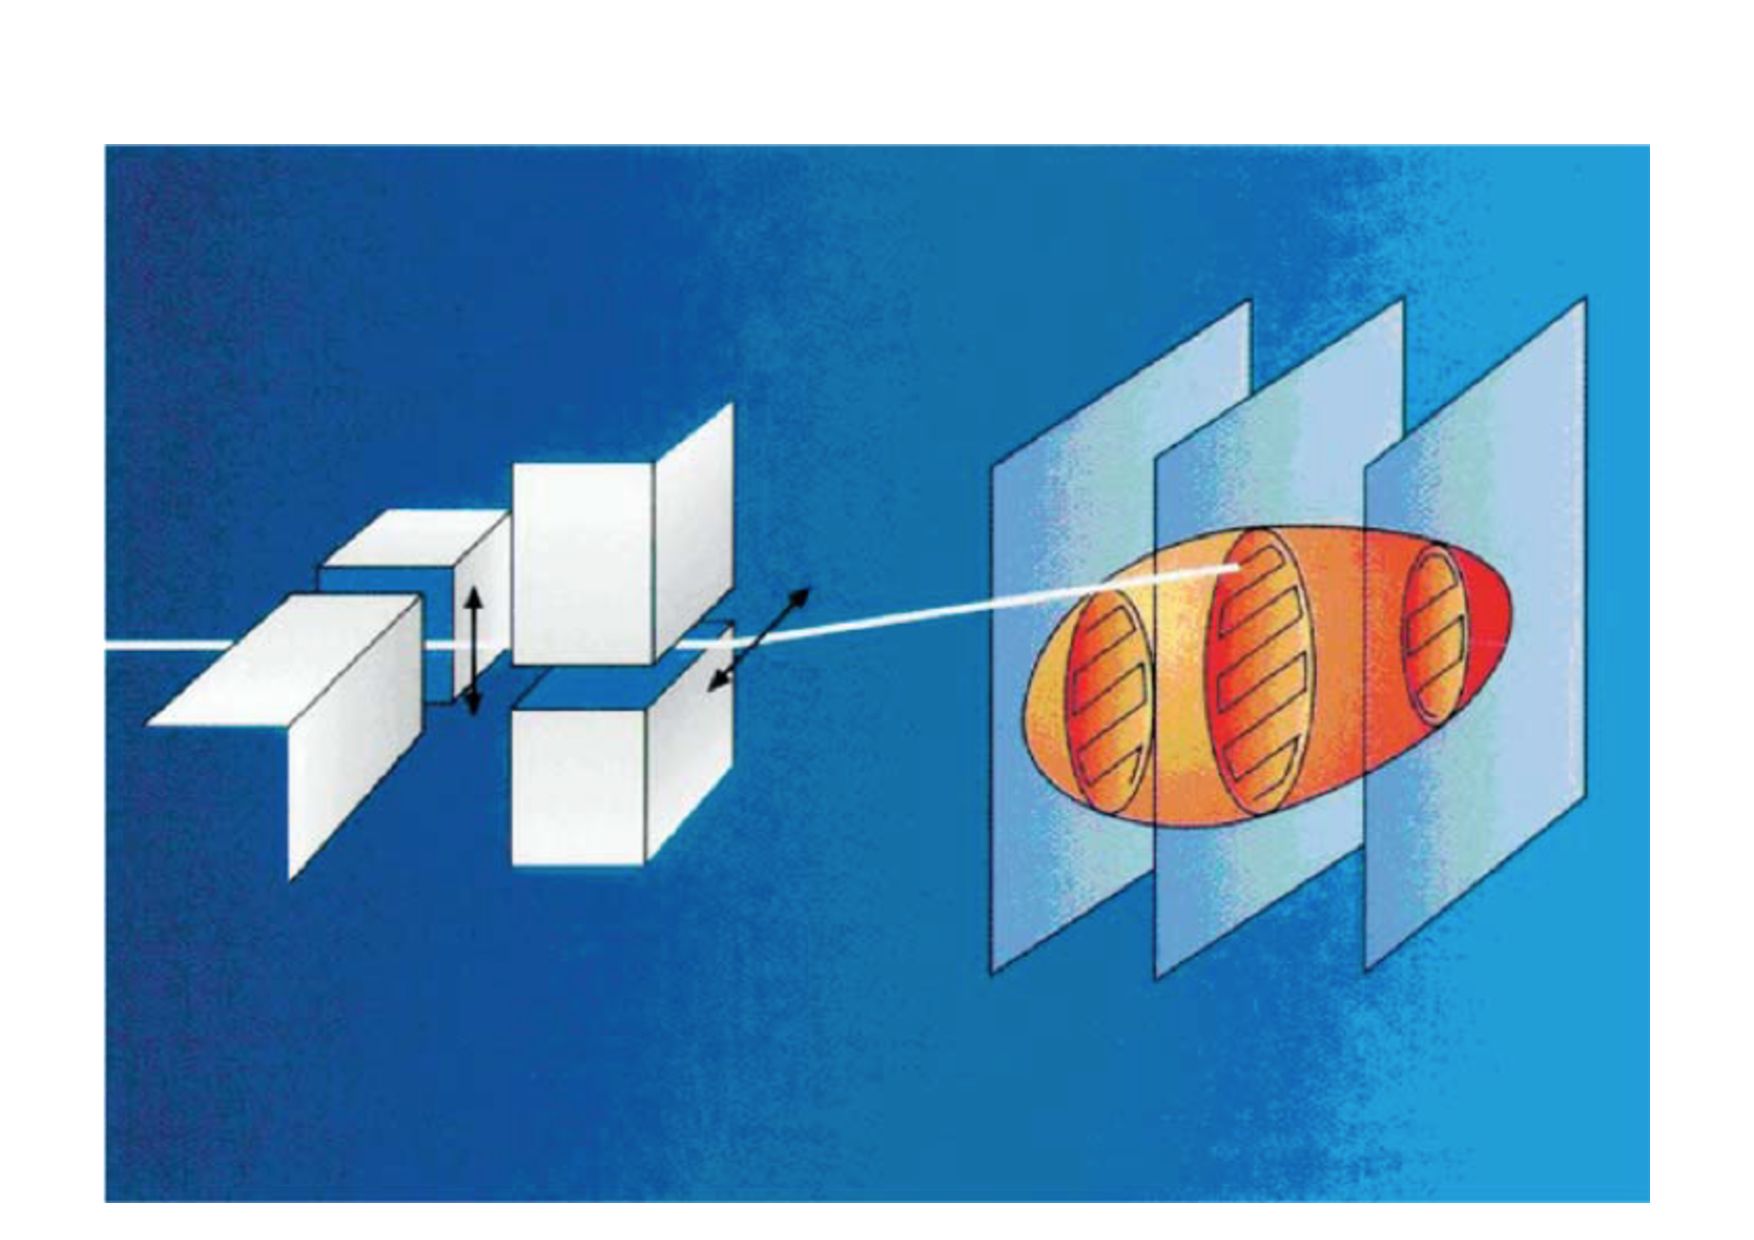
\includegraphics[width=0.7\textwidth]{03_GraphicFiles/chapter1_Introduction/activeDelivery.pdf}
\caption{Schematic view of a fully active beam delivery system. In particular, here the \gls{gsi} raster scanning system is depicted. In~\cite{Schulz-Ertner2006}.}
\label{chap1::fig::activeDelivery}
\end{figure} 

Even if this approach is demanding from the accelerator performance point of view, it brings several advantages with respect to a passive one: there is no need for patient specific equipment like collimators and compensators, and any volume can be in principle covered with a conformal dose; the dose can be adapted on a single voxel basis; the material in the beam line is minimized so that the production of secondary particles is strongly reduced. 
With such a delivery system, the term \gls{impt} has been introduced, in analogy to the \gls{imrt} techniques applied in standard photon radiotherapy.
The first so-called \enquote{spot-scanning} system was introduced at \gls{nirs}, already in the early 80's~\parencite{Kanai1983}. This first experience was soon followed by a pilot project of spot-scanning at \gls{psi}~\parencite{Pedroni1995} and by the realization of a fully 3D scanning beam system at \gls{gsi}, where the \enquote{raster-scan} technique is implemented~\parencite{Haberer1993} (with the beam moved from one voxel to the next one with no interruptions, and all points in an iso-energy slice connected together in a dense grid).
Nowadays, various companies are offering commercial scanning beam system solutions, so that a rapid spread of this convenient technique is foreseen for the next years.
 
We described till here static beam configurations, \myMarginnote{Rotating-gantries} with a fixed irradiation position. In the clinical routine, in order to further improve the target volume-to-healthy tissue dose ratio, various beam penetration angles can be foreseen, similarly to standard photon therapy (event if a reduced number of different angles is required). In addition to this, deep-seated tumors close to \glspl{oar} can require specific irradiation angles to be treated with the desired safety margins. In order to achieve this goal, two approaches are possible: rotate the patient or rotate the beam line. 
Even if the patient rotation solution has been explored in the past, several reasons are in favor of a fixed supine position, with only horizontal rotations allowed: the supine position is in compliance with the pre-treatment imaging (\gls{ct} scan) used for treatment planning (see section~\ref{chap1::subsec::treatmentPlan}); a patient rotation necessarily leads to organ motion which is undesired; the supine position is more reproducible in the different treatment fractions. As a consequence, rotating gantries have been developed to allow for the beam line displacement.    
The electron linacs employed in conventional radiotherapy are generally mounted on gantries which can rotate 360 degrees around the patient couch to select the optimum beam direction. 
Likewise, in hadrontherapy, rotating gantries solutions have been designed for both protons and heavier ions. In contrast to the compact gantries used in standard radiotherapy, the high beam magnetic rigidity (defned as the product of the bending radius and the required magnetic field strength) is a constraint on the size of these structures for proton therapy, and, much more, for heavier ion therapy. In general, the beam is first deflected away from the extraction axis, and then bent back to the patient direction with several dipoles. Moreover, quadrupoles are use to optimize the beam focusing before the treatment room. A scheme of a standard gantry desing is given in \figurename~\ref{chap1::fig::schemeGantry}. As already mentioned in section~\ref{chap1::subsubsec::accelerators}, the first gantry for protons was installed at the Loma Linda University Medical Center in 1990, followed in 1996 by the first one in Europe at \gls{psi} in 1996, which also included an upstream scanning system~\parencite{Pedroni1995}. At present most of proton therapy centers are equipped with at least one rotating gantry, generally with passive beam delivery systems.
The huge dimensions imposed by the carbon ion beam rigidity (three times bigger rigidity for 5000~MeV carbon ions with respect to 200~MeV protons) limited the implementation of such a technology in carbon therapy centers, while different technical solutions have been explored. As an example, at \gls{himac}, in a single treatment room the beam can be delivered to the patient via an horizontal and a vertical line, for the sequential treatment from different angles. The first rotating gantry system for heavy ions was installed at \gls{hit} and is now in operation: the diameter is of 13~m, for a total weight of about 700 tons (see \figurename~\ref{chap1::fig::HITgantry}).

 \begin{figure}[!htbp]
 \begin{subfigure}[t]{.49\textwidth}
\centering
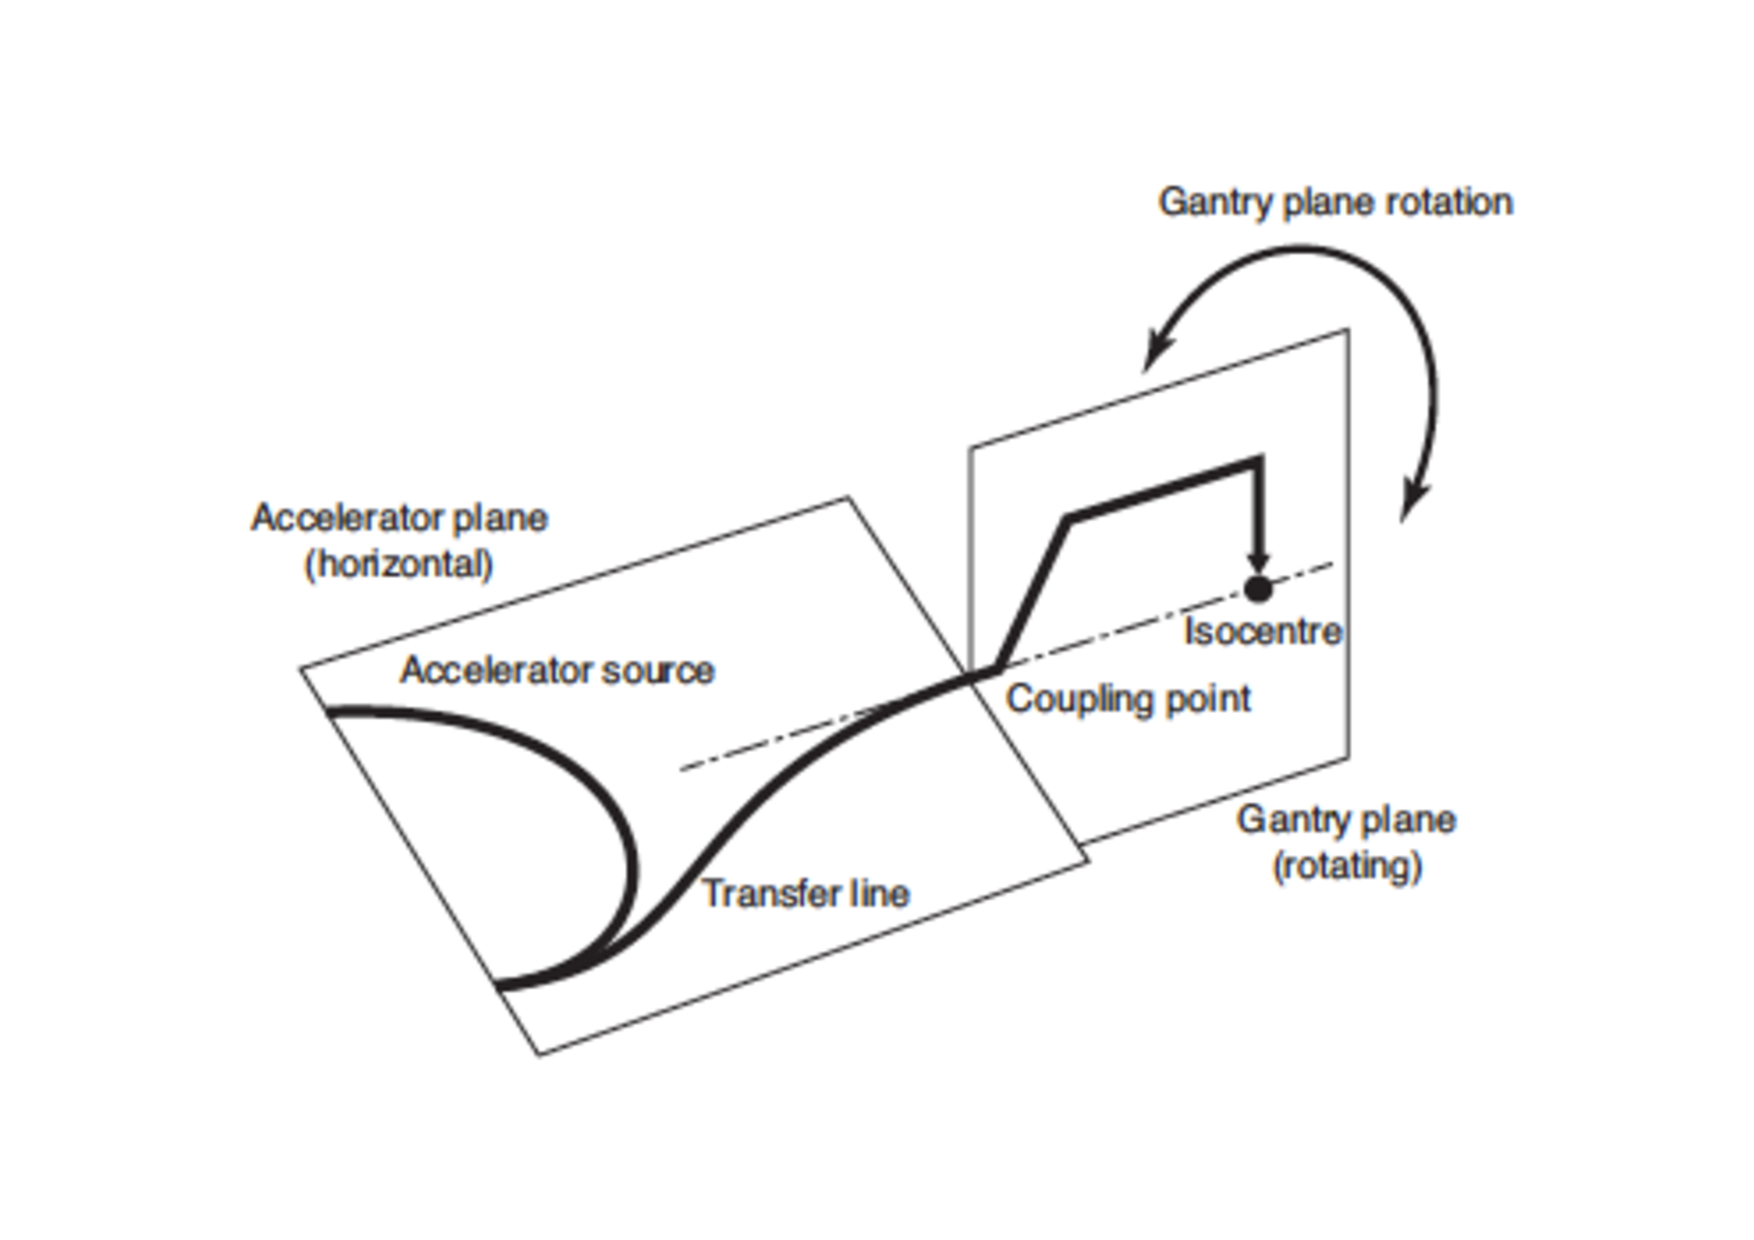
\includegraphics[width=0.92\linewidth]{03_GraphicFiles/chapter1_Introduction/scheme_gantry.pdf}	
\caption{Schematic design of a rotating gantry installed in a particle therapy center. In~\cite{Owen2014}.}
\label{chap1::fig::schemeGantry}
\end{subfigure}
 \begin{subfigure}[t]{.49\textwidth}
\centering
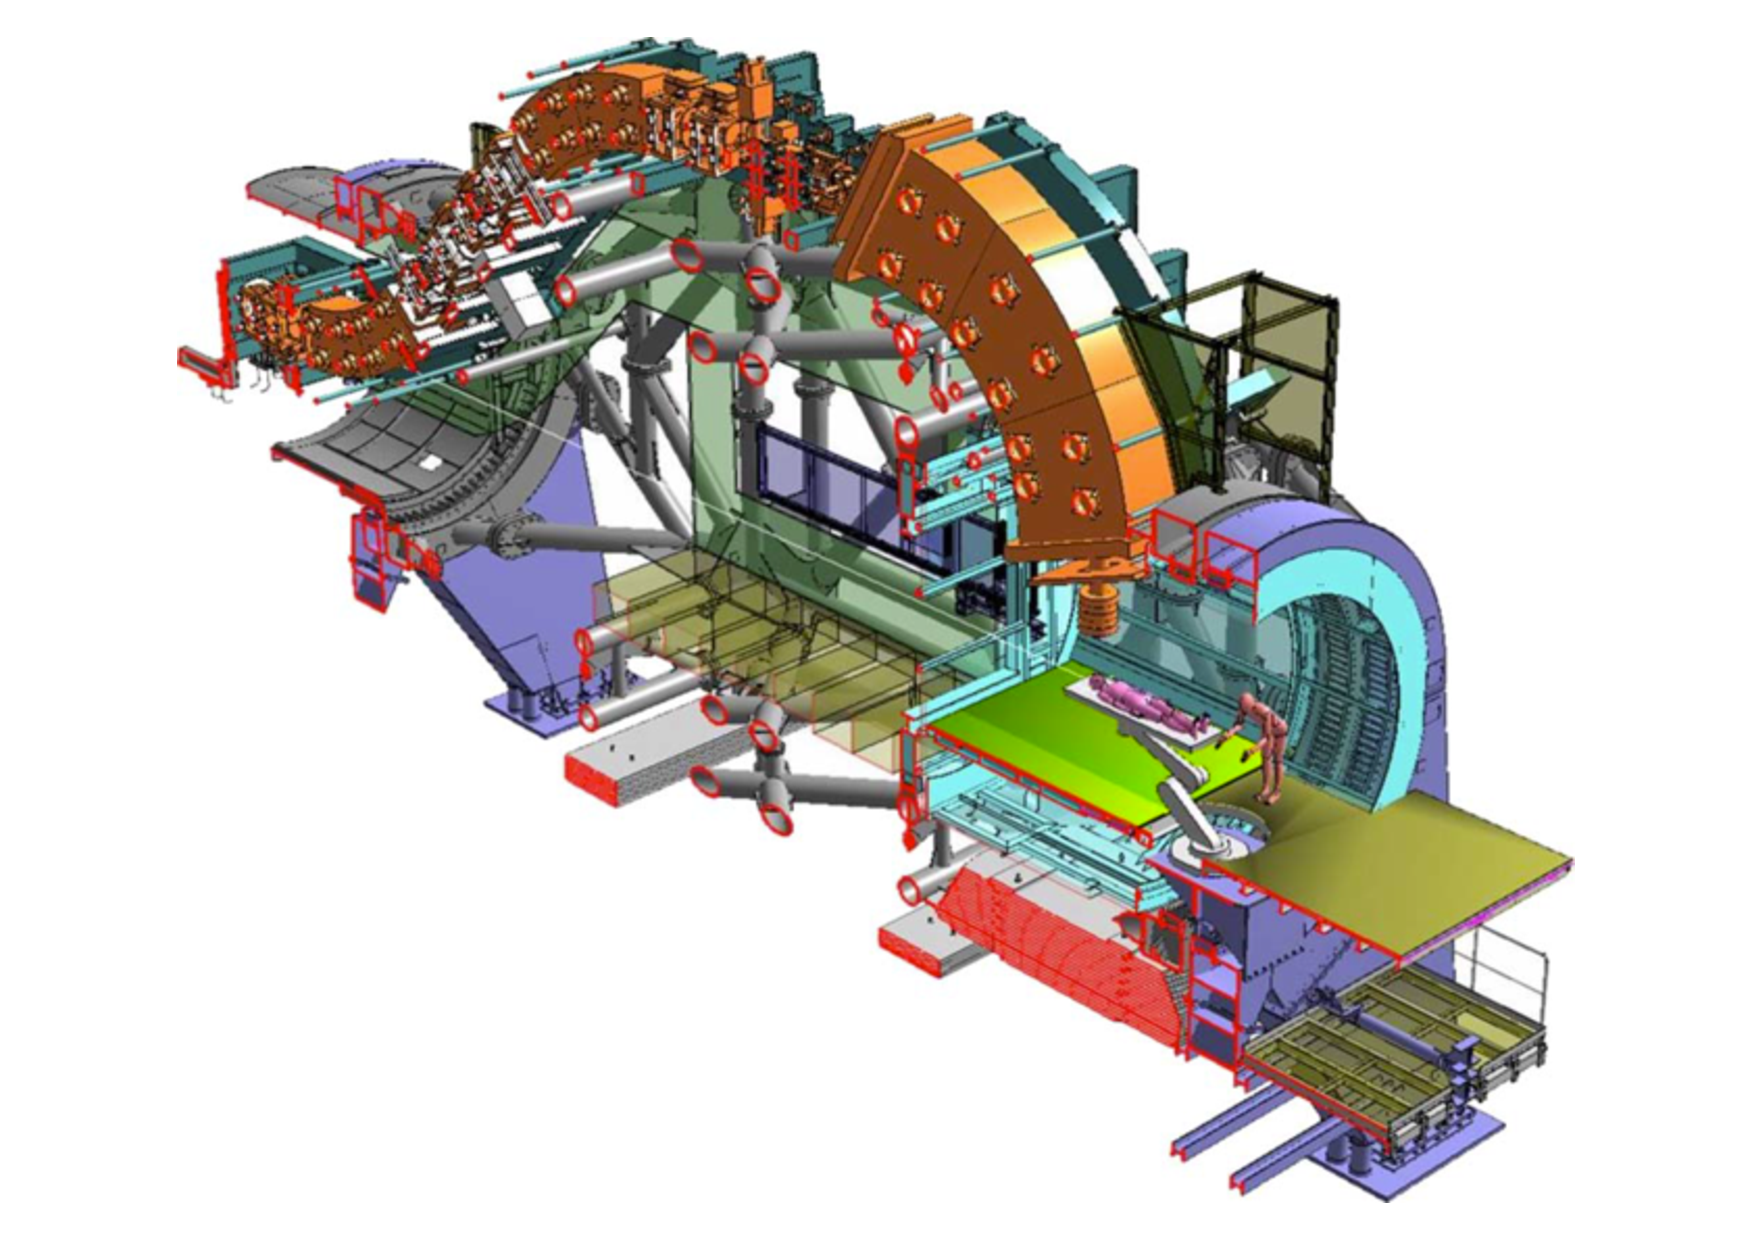
\includegraphics[width=0.99\linewidth]{03_GraphicFiles/chapter1_Introduction/HITgantry.pdf}
\caption{Scheme of the \gls{hit} ion rotating gantry. In~\cite{Schardt2010}.}
\label{chap1::fig::HITgantry}
\end{subfigure}
\caption{Schemes of a standard gantry design (left) and of the carbon-ion rotating gantry installed at \gls{hit} (right).}
\label{chap1::fig::Gantry}
\end{figure}           

Intense research efforts are dedicated to improve the gantry technology, mainly directed towards the implementation of more compact systems equipped with superconducting magnets. A first superconducting carbon ion gantry has been recently installed at \gls{nirs}, and is approximately half size with respect to the German one~\parencite{Iwata2013}.

\subsection{Treatment planning}\label{chap1::subsec::treatmentPlan}

Given the available accelerator and beam delivery system, the best possible treatment features are elaborated by the treatment planning process, which combines the clinical information about the patient with the physical an biological aspects of particle therapy. 
The treatment planning is always patient and disease-specific, and is based on imaging techniques aiming to provide the physicians with the data necessary to delineate the target volume and the surrounding \glspl{oar}. The minimal approach is represented by a pre-treatment x-ray \gls{ct} scan, providing quantitative information about the anatomical structures via photon attenuation images. As briefly outlined in the previous paragraph, it is important to record the pre-treatment images in the same conditions (patient position, fixation structures, etc.) later applied in the treatment itself. Complementary imaging devices, such as \gls{mri} and \gls{pet}~\parencite{Levy2007}, are often used in combination with \gls{ct} to improve the target definition quality, mainly in case of proximity with \glspl{oar}.
In addition to the target delineation, the physicians are also in charge of the therapy prescription, which includes the total dose to be delivered to the \gls{ptv}, the dose limits for the surrounding tissues, and the fraction planning.
All the listed information are the input for the \gls{tps} \myMarginnote{Treatment-Planning System}, which makes the connection between the prescribed dose distribution and the beam acceleration and delivery devices. The physicists and clinicians use the \gls{tps} to define all the treatment beam-specific features such that the clinical prescription is satisfied at the maximum extent. The software output details the beam entrance ports to be used (in terms of gantry positions, if a gantry is available), the beam ranges and intensities, the irradiation scheme in terms of dose-per-voxel, and, more generally, the expected dose distribution in the patient, which allows to quantify the ~\gls{tcpr} and the probability of complications to
the normal tissues.
As the whole planning process is based on x-ray \gls{ct} scans,  \myMarginnote{From \gls{hu} to \gls{rsp}} providing photon beam attenuation images, a relationship between the \gls{ct} values and ion~\gls{rsp} is needed. The \gls{ct} values are expressed in \gls{hu}, defined as

\begin{equation}
\mathrm{CT\,value}(\vec{x}) =1000 \times \frac{\mu (\vec{x})-\mu_{W}}{\mu_{W}}
\label{chap1::eq::HU}
\end{equation}
where $\vec{x}$ is the considered location, $\mu(\vec{x})$ the x-ray absorption coefficient in tissue, $\mu_{W}$ the one in water as reference. Water is always used as reference medium, in particular through the concept of \gls{wepl}. There is not a functional relationship between the two quantities, and systematic studies have been carried out at \gls{psi} for protons~\parencite{Schneider1996, Schaffner1998}. For carbon ions, similar investigtions have been performed at \gls{nirs}~\parencite{Matsufuji1998, Kanematsu2003} and \gls{gsi}~\parencite{Jakel2001, Rietzel2007}, and experimental verification has been obtained via measurements on animal tissues. In \figurename~\ref{chap1::fig::HU} the data of a look-up table for the conversion of \gls{hu} into carbon ion \gls{wepl} are plotted in the \gls{hu} range of relevant biological tissues.

 \begin{figure}[!htbp]
 \begin{subfigure}[t]{.49\textwidth}
\centering
\includegraphics[width=0.92\linewidth]{03_GraphicFiles/chapter1_Introduction/HounsfieldUnits.pdf}	
\caption{Hounsfield look-up table for carbon ion treatment planning, based on the data collected at \gls{gsi} and reported in~\cite{Jakel2001}. In~\cite{Rietzel2007}.}
\label{chap1::fig::HU}
\end{subfigure}
 \begin{subfigure}[t]{.49\textwidth}
\centering
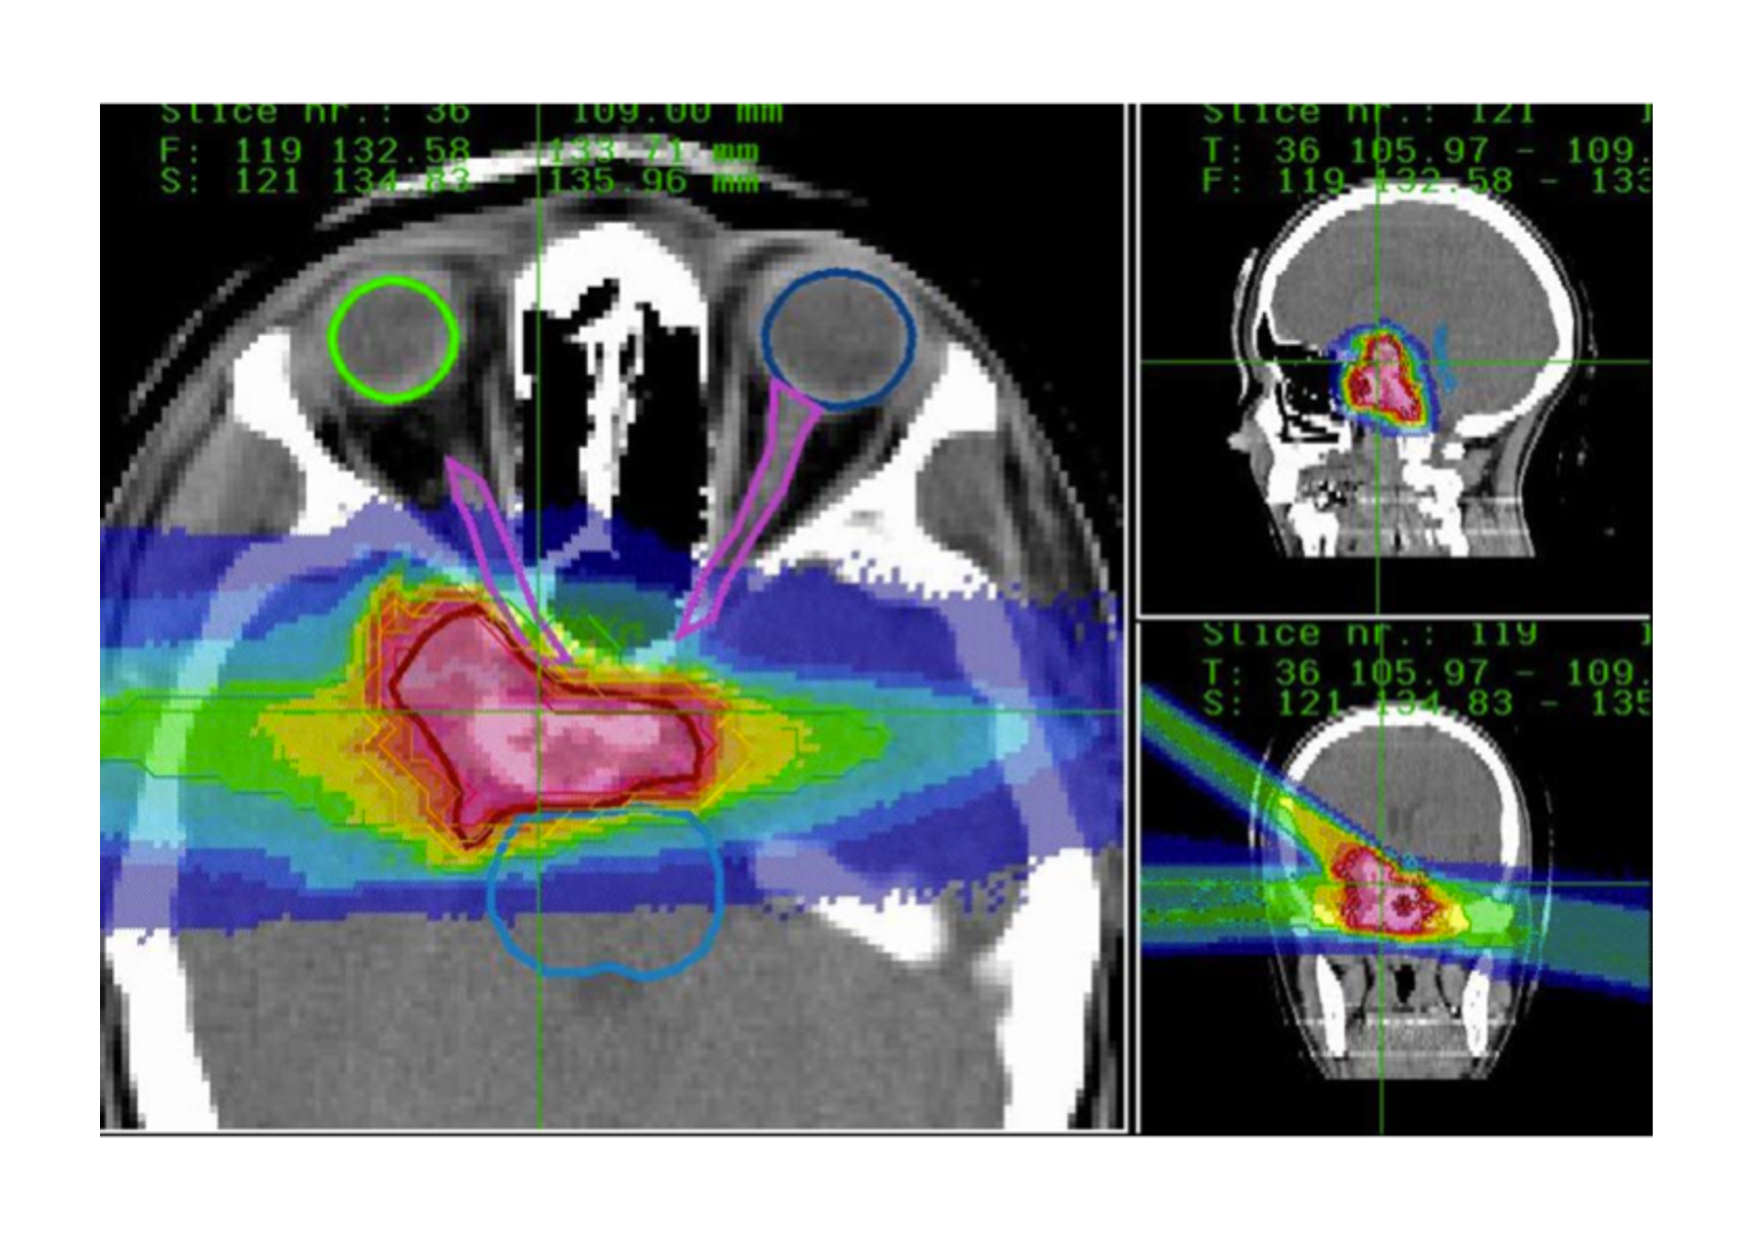
\includegraphics[width=0.92\linewidth]{03_GraphicFiles/chapter1_Introduction/TRIPplan.pdf}
\caption{Biologically effective dose distribution for the treatment of a skull base tumor, optimized with the \gls{tps} TRiP~\parencite{Kramer2000} at \gls{gsi}. In~\cite{Schardt2010}.}
\label{chap1::fig::}
\end{subfigure}
\caption{The treatment planning system process is based on anatomical information about the patient, given by \gls{ct} scans, and physician treatment prescription. The \gls{ct} values must be converted to \gls{rsp} and tabulated experimental data are used (left), while biological dose calculation models are applied to optimize the biological dose distribution to be delivered during the treatment (right).}
\label{chap1::fig::TPS}
\end{figure}           

The conversion factors are tabulated and implemented in the main \glspl{tps}, but several studies are still ongoing in order to optimize the calibration accuracy (as an example, see~\cite{Inaniwa2018}). As highlighted in several research work, this is one of the main source of uncertainty affecting proton and carbon ion range prediction and, so, treatment preciseness. Possible investigated solutions to reduce systematic uncertainties in the \gls{rsp} determination related to the Hounsfield unit conversion are represented by \gls{pct} and dual energy x-ray \gls{ct}~\parencite{Yang2010}. Further details will be given in section~\ref{chap1::subsec::uncertainty}.
In addition to the beam range determination, \myMarginnote{Biological dose modeling} the \gls{tps} software must also deal with biological dose calculations. Indeed, as highlighted in section~\ref{chap1::subsec::bioEffects}, charged particles differ from photons in their radiobiological properties and effects. Notwithstanding the 10-20\% \gls{rbe} variations verified for protons with varying \gls{let} along the path in the patient tissues, a practical constant value of 1.1 is generally used in clinics~\parencite{Paganetti2002, ICRU2007}. This value corresponds to the average \gls{rbe} at mid \gls{sobp} overall dose levels. As mentioned in section~\ref{chap1::subsec::bioEffects}, several studies are ongoing in the last years with the aim of optimizing the biological models and applying a variable proton \gls{rbe} in clinics, and the topic is still open to discussion in the expert community~\parencite{Paganetti2013, Paganetti2014, Unkelbach2018, Luhr2018, Willers2018}. A different approach must be applied to heavy ions (carbon ions in particular), given the much stronger dependence of their \gls{rbe} on the various parameters listed in section~\ref{chap1::subsec::bioEffects}. Focusing on carbon ions, treatment plans are generally optimized using the so-called \gls{rbe}-weighted dose, calculated according to verified models based on experimental data. Two main models are nowadays implemented in clinical practice. On one side, the Japanese centers use a model developed at \gls{nirs}, based on in vitro cell killing experiments on human salivary glands and neutron irradiation experience gathered at \gls{himac}, as well as on the application of the \gls{lq} model~\parencite{Matsufuji2007}. Recently, a modified \gls{mkm} has been introduced in order to optimize the plans to active scanning with ion beams~\parencite{Inaniwa2015}. On the other side, a specific biophysical model has been developed in Germany at \gls{gsi}, called \gls{lem}, and it is now used in the clinical centers in Germany, Italy and China. Its main idea is to transfer known cell-survival data for photons to ions, assuming that the difference in biological efficiency arises only from a different pattern of local dose deposition along the primary beam~\parencite{Kramer2000, Jakel2001a}.
The two models have been verified to give comparable results, in agreement with the measured \gls{rbe}, with in-vitro experiments on mice cells~\parencite{Uzawa2009}, while different predictions are obtained when different treatment schemes on different tissues are studied~\parencite{Fossati2012, Steinstrater2012}. The definition of a common effective dose prediction methods is ongoing: this will allow for comparative studies of clinical results and for an improved collaboration of the few ion treatment centers operating all over the world.
These biological models are mainly applied for the planning of active scanning treatments, for which the target volume is previously divided into slices: the dose is then optimized for iso-range slices. In contrast, for passive beam delivery systems, the plan optimization is generally reduced to the study and production of the patient-specific beam modulators. 
In the future, biology-guided forms of particle therapy can be foreseen; the \gls{rbe} variations, instead of being an issue for which corrections are needed to the treatment planning, could be used to the treatment effectiveness advantage.  
Focusing on the possible direction of improvements in the future of treatment planning \myMarginnote{Treatment of moving organs}, the research efforts are concentrated in the last years also on another fundamental topic: the treatment of moving organs. It is clear that the well-defined ion range and narrow dose peak makes them potentially more sensitive towards inter- and intra-fractional organ motion, as highlighted in~\cite{Phillips1992, Bert2008, Engelsman2013} and~\cite{Thornqvist2013}, as an example. Concerning the organ displacement between following fractions, it can be corrected by more frequent imaging scans, ideally a new one before every treatment fraction, in order to adapt the treatment planning to weight variations, target size modifications and similar anatomical effects. The organ movement caused by the respiratory cycle requires more complex strategies to be taken into account for the treatment plan and delivery. The respiratory motion patterns are genarally complex and not regular, involving translational and rotational displacements. Several strategies to mitigate the effect of organ motion are being investigated, some of them directly coming from the experience gathered in \gls{imrt}. As well summarized in~\cite{Schardt2010}, among these strategies it is worth to mention rescanning of repainting techniques, based on the average effect of several irradiations with reduced beam fluence on the same iso-range slices; gating techniques, which aims to correlate the irradiation active time to a continuous monitoring of the respiration cycle; tracking, which requires a 3D compensation of the target motion in real-time, particularly adapted for scanning techniques. Some of the cited techniques, or combinations of them, are being tested and are now at the validation stage, but there still wide room for improvements towards the application of 4D treatment planning~\parencite{Graeff2013, Bert2017}. Further information about this topic  can be found in a recent review by Kubiak~\parencite{Kubiak2016}.    
Range predictions, biological modeling and organ motion are only some of the sources of uncertainties affecting the planning and delivery of ion therapy treatment, detailed in section~\ref{chap1::subsec::uncertainty}; for this reason, safety margins \myMarginnote{Safety margins} are applied in clinics for the definition of the irradiation target volume and the quantification of the planned dose. In the actual clinical routine, the \gls{ptv} is a geometrical extension of the so-called \gls{ctv} and is delineated in order to account for treatment uncertainties. Safety margins are also applied in standard x-ray therapy~\parencite{McKenzie2000}, where under- or over-shooting errors have limited effects with respect to ion beam therapy. As highlighted in~\cite{Albertini2011}, the application of safety margins is useful to improve the treatment plan robusteness in case low dose gradients are applied, while the effect results marginal for highly modulated \gls{impt}. At present, in order to account for the overall effects of all source of uncertainties in the range prediction (\gls{mcs}, beam energy straggling, imaging tools accuracy and calibration, biological effects, patient positioning and organ motions), margins up to 3.5\% + 3~mm can be applied around the \gls{ctv}~\parencite{Paganetti2012}, mainly based on Monte Carlo or analytical dose calculations which result in clinically compatible predictions. 

In the following paragraph, the uncertainties related to ion therapy treatment are discussed in details, with particular care devoted to possible clinical solutions.

\subsection{Ion beam therapy uncertainties and treatment monitoring}\label{chap1::subsec::uncertainty}
Heavy charged particles are suitable for cancer radiation therapy given the better achievable dose conformity and the reduced energy deposit in tissues surrounding the target with respect to standard photon treatment techniques. These advantageous features directly derives from the nature of ion interactions in matter, described in section~\ref{chap1::subsec::Physics}, which determine a peculiar depth dose profile characterized by a finite range and a energy deposit (dose) peak (Bragg peak). In order to accurately predict the ion range and, more generally, the dose distribution delivered during a clinical treatment, all the possible ion interactions in matter must be considered. This prediction is associated with considerable uncertainties due to imaging precision, patient setup, anatomical variations and motions, beam delivery system accuracy, dose calculation approximations and biological considerations~\parencite{Paganetti2012}. Ideally speaking, a perfect knowledge of the beam and target structure and perfect evaluation of all the parameters involved in the dose determination would result in the optimal way to treat a deep-seated tumor, with a reduced dose delivered to the surrounding healthy tissue (even close to \glspl{oar}) with limited fields of irradiation, and a dose accurately concentrated to the tumor volume. The actual clinical routine must face limitations in beam production and control as well as in patient composition evaluation, which causes the need for approximated treatment planning and the setup of treatment safety margin (see section~\ref{chap1::subsec::treatmentPlan}), limiting the full exploitation of this treatment technique potential. In this section, an overview of the different sources of uncertainties affecting ion therapy treatments is given, and the solutions, already implemented or under study, are presented, with particular attention focused on ion range monitoring techniques, main topic for this thesis.
All the mentioned sources of uncertainties associated to hadrontherapy treatment converge in a considerable spread in the beam effective range with respect to the predicted one. Treatment planning systems are able to accurately model range straggling and \gls{mcs} broadening along the beam path in water~\parencite{Hong1996}, but the prediction accuracy has limitations when translated to patients. As highlighted in~\cite{Schlegel2008}, a precise determination of the primary ion penetration depth is essential in order to rely on particle therapy treatments, much more than for standard photon treatments. The reason is schematically presented in \figurename~\ref{chap1::fig::rangeUnc}.

\begin{figure}[!htbp]
\centering
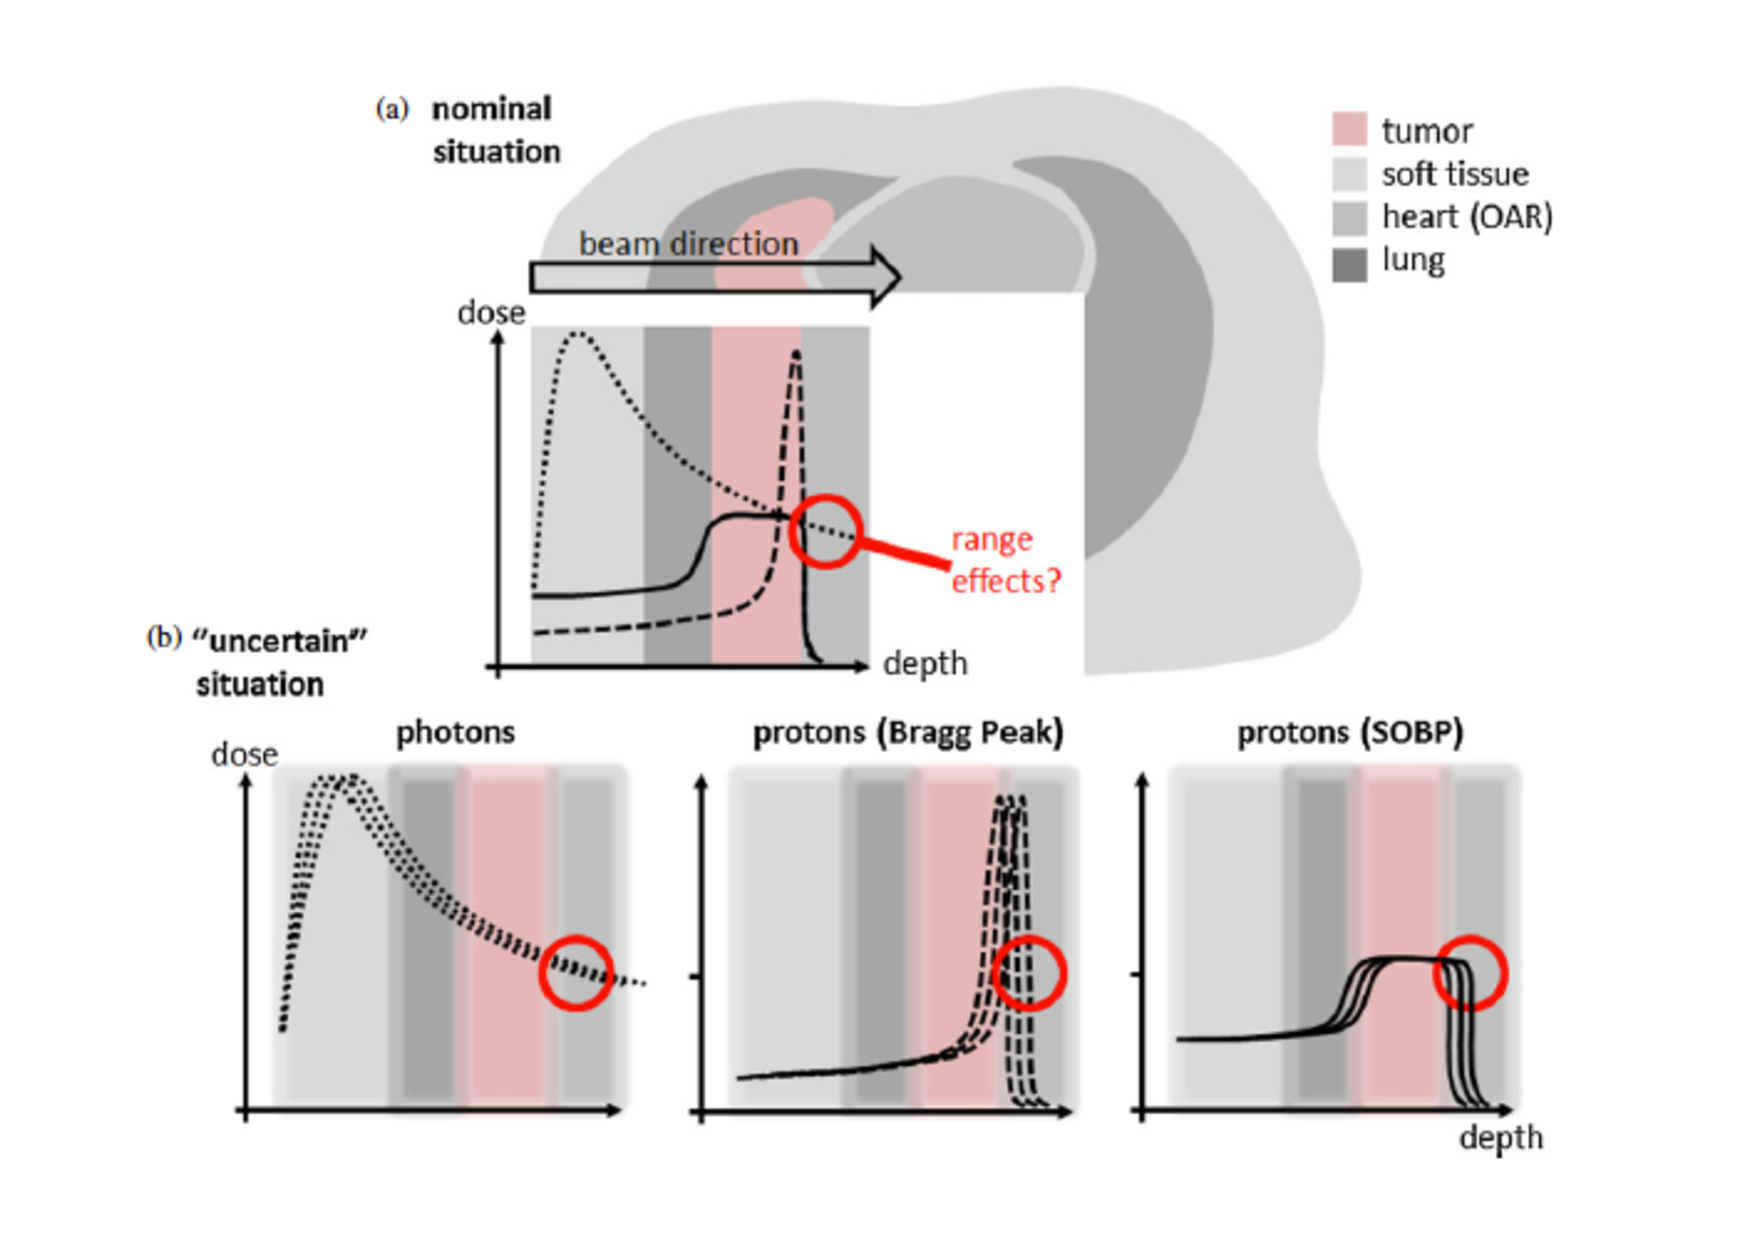
\includegraphics[width=0.7\textwidth]{03_GraphicFiles/chapter1_Introduction/rangeUnc.pdf}
\caption{Schematic view of the potential benefit due to the depth-dose features of protons as compared to photons (a) and influence of range uncertainties on photon irradiation and proton prinstine and spread-out Bragg peak. In~\cite{Knopf2013}.}
\label{chap1::fig::rangeUnc}
\end{figure} 

In the top panel of \figurename~\ref{chap1::fig::rangeUnc} the ideal treatment configuration is shown, with the pristine Bragg peak located at the distal limit of the \gls{ptv} (dashed line) and the \gls{sobp} covering the whole tumor volume (solid line); the two proton irradiation methods are compared to the photon dose profile (dotted line), which release the maximum of the dose in the entrance region and it is not capable of sparing the tissues surrounding the tumor volume, before and beyond the tumor in the beam direction. In the bottom line of the same figure, the effect of range uncertainties are represented: from left to right, in case of photon dose profile shifts, the modification in the dose delivered to healthy tissues is relatively limited, the main effect being a shift in the dose peak in the entrance region; for a monoenergetic Bragg peak, a shift in the peak position can result in both an under-irradiation of malignant tissues and a dose maximum located in soft healthy tissues; the same effect is present for the \gls{sobp}, with the only advantage of a reduced under-irradiation of the tumor region. It is clear from this simple case how the extremely sharp dose gradient provided by heavy charged particles must be accurately controlled in order to fully profit of its beneficial effect in treating cancer. 
As mentioned, an exact range calculation is extremely difficult to be obtained in human tissues. As described in section~\ref{chap1::subsec::treatmentPlan}, the treatment planning is at present based on a pre-treatment \gls{ct} scan which is generally acquired only before the first treatment fraction. The \gls{ct} image accuracy is indeed the first source of uncertainty in range calculation \myMarginnote{\gls{ct} uncertainty}. The limitations in the imaging precision (mainly due to image noise - see~\cite{Chvetsov2010}) and the reconstruction artifacts (which can be relevant in presence of metal implants as verified in~\cite{Jakel2007, Newhauser2007}) already affect the reference data set. Small but not negligible effects are also related to the \gls{ct} resolution~\parencite{Espana2011}. The obtained \gls{ct} data must be then converted from x-ray attenuation values (\gls{hu}) related to water to relative ion stopping power (see section~\ref{chap1::subsec::treatmentPlan}). The conversion is based on calibration curves~\parencite{Schneider1996, Schneider2000}, generally obtained with \gls{ct} scans of tissue phantom materials with known density and elemental composition. These curves are affected by uncertainties, to be added to the fact that the actual conversion is dependent on the material composition: same x-ray attenuation values can correspond to different relative stopping power, or vice versa. In addition to this, the conversion may depend on the specific \gls{ct} scanner, as shown in~\cite{Ainsley2014}. Several studies have highlighted the magnitude of such uncertainties, which varies, for example, in the range 1-2\% from soft tissues to bones for protons~\parencite{Schaffner1998b}, which is translated in range possibile discrepancies of 1-3~mm. Specific studies have also been conducted on animal fresh tissues in order to otpimize the \gls{ct} calibration for carbon ion treatments~\parencite{Rietzel2007}. In total, uncertainties of the order of 3\% are generally considered to take into account the described imaging limitations~\parencite{Moyers2001}. It has been proven that dual-energy \gls{ct} can improve material composition information~\parencite{Bazalova2008, Yang2010, Hunemor2014, Wohlfahrt2018} and the resulting range uncertainties can be reduced, in particular for carbon ion therapy~\parencite{Hunemor2014}. A possible solution to further reduce the errors related to the \gls{hu} values conversion is the implementation of direct density measurements techniques, where the treatment beam is also used for imaging purposes giving direct access to stopping power data. This possibility was discussed since the late sixties~\parencite{Koehler1968}, and the technological advancements (mainly in data acquisition systems and detection techniques) recently allowed to obtain promising results in the last years. In addition to the advantageous removal of the data conversion stage, the so-called ion radiography brings other benefits to the treatment side, with the possibility of performing position verification with fast scans just before the treatment delivery~\parencite{Schneider1995}, as well as on the patient side, given the reduced dose necessary for a complete scan with respect to standard x-ray \gls{ct}~\parencite{Schneider1995}. Further details about this imaging technique are given in the dedicated section~\ref{chap1::subsubsec::particleCT}.
Till here the uncertainties directly coming from the treatment planning process have been described, and can be considered as systematic errors, reproduced unchanged for every delivered fraction of the treatment. Conversely, stochastic uncertainties emerge at the treatment delivery level and affect the planned range with random variations. The majority of treatment planning system operating in clinics are based on analytical calculations relying on \gls{wepl} data, not able to account for complex geometries. In presence of tissue inhomogeneities \myMarginnote{\gls{mcs} range degradation}, \gls{mcs} causes what is generally referred to as a degradation in the distal fall-off of Bragg peaks~\parencite{Urie1986}, in particular in proximity of high-density gradients.  Accurate modeling of \gls{mcs} is then strictly required for correct range predictions~\parencite{Schuemann2014}. The patient anatomical configuration\myMarginnote{Patient anatomy changes} plays a major role not only on a single fraction basis, but also in different fractions. Conventional fractionation schemes foresee treatments which can last for several weeks; the patient anatomical characteristics can experience significant changes, such as tumor mass reduction, weight loss or gain~\parencite{Albertini2008}, modifications in the filling of internal cavities. It is clear that such variations introduce further shifts in the predicted ion range, which can be different from fraction to fraction. Moreover, in different fractions, slight differences in the delivered ion energy are possible, with small but not negligible effects. 
Moving on but always referring to static anatomy issues, the patient setup in the treatment room is another source of uncertainty which can cause discrepancies between the planned and the delivered dose distribution, as shown for example in~\cite{Fattori2014}. 
Furthermore, in particular for the treatment of tumors in the thorax, organ motion \myMarginnote{Organ motion dose blurring} is an important source of dose delivery errors. Focusing on lung cancers, which are already difficult to be precisely targeted due to the low lung density (3 times lower than water), the respiratory motions are hard to be modeled and cause an overall blurring of the dose distribution and severe local range variations due to the high-density gradient between dense tumor tissues and low-density lung tissue. Important research efforts are devoted to the optimization of the treatment of moving organs, as explained in section~\ref{chap1::subsec::treatmentPlan}. In particular, for active scanning delivery techniques, potentially powerful if synchronized with the movements of the target areas, an interplay effect involving beam and organ motion can affect the dose homogeneity and must be minimized~\parencite{Dowdell2013, Grassberger2015}.
To conclude the list of source of uncertainties affecting ion beam therapy treatment planning and delivery, it is worth to mention the contribution of biological effects \myMarginnote{Biological effects}. For protons, a generic constant \gls{rbe} value is generally used in clinics to relate proton dose to photon dose, while it has been verified how the biological effectiveness varies along the beam path, in particular at varying \gls{let}. In \gls{sobp}, the increasing \gls{let} at decreasing primary residual energy is compensated by a reduction of the proton fluence, in order to obtain an homogeneous dose distribution. The increase in \gls{let} causes an increase in the\gls{rbe} which is not considered and result in a shift in the biologically effective range, estimated in $\sim$1-2~mm~\parencite{Paganetti2000, Robertson1975, Wouters1996}. Heavier ion therapy planning system already account for \gls{rbe} variations to prescribe a conformal dose distribution, but the prediction process is not error-free. Moreover, the dose distribution delivered with heavy ion irradiation is also characterized by the peculiar tail beyond the Bragg peak cause by the nuclear interaction fragments; a correct prediction of the nuclear interaction channel becomes significant, and it is at present not accurate enough to point the beam towards critical structures and fully profit of the narrow dose peak.
The optimization of treatment planning system is focused, in the last years, on Monte Carlo-based dose plans, which can reduce the listed uncertainties, and rely on the continuous progress of physical and biological modeling. A complete overview about this topic is given in~\cite{Paganetti2012} for the case of protons. In table~\ref{chap1::tab::uncertainties}, originally presented in~\cite{Paganetti2012} and here reported with the modifications which can be found in~\cite{Durante2016}, the sources of uncertainties in the proton range are reported with an estimated of their relative contribution with and without the application of Monte Carlo optimization techniques.

\begin{table}[!htbp]
\centering
\caption{Estimated magnitude of range uncertainties separated for the various sources, and potential benefit provided by Monte Carlo simulations. The estimates are based on data in~\parencite{Matsufuji1998, Schaffner1998, Chvetsov2010, Bichsel1992, ICRU1993, Kumazaki2007, Espana2010, Urie1986, Sawakuchi2008, Bednarz2010, Wouters1996, Robertson1975, Paganetti2000}. Table reproduced from~\cite{Durante2016}.}
\label{chap1::tab::uncertainties}
\begin{tabular}{m{6cm} P{3.6cm}  P{3.6cm}}
\toprule
\rowcolor{myColorMainA!20} 
\textbf{Source of range uncertainty in the patient}& \textbf{Range uncertainty w/o Monte Carlo (\% or mm)} & \textbf{Range uncertainty with Monte Carlo (\% or mm)} \\
\midrule
\underline{Independent of dose calculation}: & & \\
\hspace{0.2cm} Measurement uncertainty in water & $\varpm$ 0.3~mm & $\varpm$ 0.3~mm \\
\hspace{0.2cm} for commissioning  & & \\
\hspace{0.2cm} Compensator design & $\varpm$ 0.2~mm & $\varpm$ 0.2~mm \\
\hspace{0.2cm} Beam reproducibility & $\varpm$ 0.2~mm & $\varpm$ 0.2~mm \\
\hspace{0.2cm} Patient setup & $\varpm$ 0.7~mm & $\varpm$ 0.7~mm \\
\underline{Dose calculation}: & & \\
\hspace{0.2cm}  Biology & + $\sim$ 0.8\% & + $\sim$ 0.8\% \\
\hspace{0.2cm}  \gls{ct} images and calibration & $\varpm$ 0.5\% & $\varpm$ 0.5\% \\
\hspace{0.2cm}  \gls{ct} conversion to tissue & $\varpm$ 0.5\% & $\varpm$ 0.2\% \\
\hspace{0.2cm} (excluding I-values) & & \\
\hspace{0.2cm}  \gls{ct} grid size & $\varpm$ 0.3\% & $\varpm$ 0.3\% \\
\hspace{0.2cm}  Mean excitation energy (I-values) & $\varpm$ 1.5\% & $\varpm$ 1.5\%  \\
\hspace{0.2cm} in tissues & & \\
\hspace{0.2cm}  Range degradation: complex & - 0.7\%  & $\varpm$ 0.1\%  \\
\hspace{0.2cm} in-homogeneities  & & \\
\hspace{0.2cm}  Range degradation: local lateral & $\varpm$ 2.5\% & $\varpm$ 0.1\%\\
\hspace{0.2cm} in-homogeneities  & & \\
\midrule
\hspace{0.5cm}  \underline{Total} (excluding biology and & 2.7\% $\varpm$ 1.2~mm & 2.4\% $\varpm$ 1.2~mm \\
\hspace{0.7cm} lateral in-homogeneities) & & \\
\hspace{0.5cm}  \underline{Total} (excluding biology) & 4.6\% $\varpm$ 1.2~mm  & 2.4\% $\varpm$ 1.2~mm  \\
\bottomrule
\end{tabular}
\end{table}      

As mentioned in section~\ref{chap1::subsec::treatmentPlan}, the current approach to deal with range uncertainties directly comes from standard x-ray radiation therapy and involves the setting of margins around the target volume. The margins are generally determined analytically and results to be larger in the distal end of the target volume to account for range shifts, while smaller margins are applied laterally to include beam penumbra uncertainties. The field arrangement is another applied mitigation of the problem~\parencite{Lomax2001}, in particular in proximity of \glspl{oar}. For example, lateral fields can be used instead of distal ones. 
Notwithstanding the several solution used, \textit{in-vivo} verification of the delivered range is still a pressing desire in the clinical community. Standard imaging devices are commonly used to monitor photon therapy treatment, where the delivered beam is not stopped in the patient. On the contrary, ion beams do not exit the patient body, so that monitoring techniques can only be based on secondary radiation or indirect measurements. An exception is represented by implanted devices, proposed for the dose and range measurements, briefly discussed in section~\ref{chap1::subsec::rangeComplTechniques}.
As highlighted in~\cite{Parodi2015}, the monitoring should be ideally in three-dimensions on-line, time-resolved and in real-time, in order to allow for a prompt detection of severe deviations between prescribed and delivered dose, and eventually for the interruption of the beam delivery. A number of different approaches have been proposed in the last years, and significant research efforts are dedicated to this specific point by several groups all over the world. In particular, nuclear reactions products are deeply investigated as a source of information about the beam range. In the following sections, after a paragraph devoted to charged particle \gls{ct}, the main techniques implemented for ion range monitoring purpose or at present under study are described, and the current available or future instrumentation is presented. In chapter~\ref{chap::2}, the attention will be focused on the detection of \glspl{pg}, central topic of this thesis, and a detailed overview of the state of the art of this particular monitoring techniques is provided.                


\subsubsection{Charged particle CT}\label{chap1::subsubsec::particleCT}

\subsubsection{Positron Emission Tomography}\label{chap1::subsubsec::RangePET}
\gls{pet} is at present the only method clinically implemented for ion range verification~\parencite{Hishikawa2002, Enghardt2004, Parodi2007, Bauer2013}. \gls{pet} techniques are based on the same principle as the ones employed in nuclear medicine diagnostics (see section~\ref{chap1::sec::NuclearMed}): in particular, for the application in ion beam range monitoring, \gls{pet} machines aim to detect the two back-to-back 511~keV photons produced by the annihilation of positrons (created by the emitter fragments of nuclear reactions) with patient electrons, resulting in a delayed radiation which should be detected with time coincidences, allowing for an intrinsic background reduction. Nevertheless, the monitoring with positron emitters secondary signal must deal with a limited count rate compared to medical imaging \gls{pet}, with the lifetime of emitters providing a delayed information that implies the signal integration over a whole treatment fraction (not a single spot or group of spots), with physiological washout effects depending on the emitters lifetime.

IN-BEAM, IN-ROOM, OFF-LINE PET. 

Even if the only available and functional range monitoring system in a clinical center is based on this technique~\parencite{Enghardt2004}, several clinical experience with commercial or adapted PET system already shown intrinsic limitations mainly connected to the ring geometry (not directly applicable to the treatment monitoring due to the presence of the beam) or in general to geometrical constraints limiting the field of view and the resulting system global efficiency and spatial accuracy (the limited detection angle generates artifacts in the final image)~\parencite{Parodi2015}. The research is ongoing and new results are expected for the next years thanks to the introductions of new systems with adapted geometries, to the improvements in acquisition and reconstruction techniques and to the clinical introduction of time-of-flight systems, intrinsically able to improve the detector spatial resolution via interaction time information, and depth-of-interaction reconstruction, which will allow for a more precise spatial reconstruction for reduced angular artifacts effects.

\subsubsection{Prompt-gamma detection}\label{chap1::subsec::PGgeneral}

\subsubsection{Interaction vertex imaging}\label{chap1::subsec::IVI}

\subsubsection{Other techniques}\label{chap1::subsec::rangeComplTechniques}




\section{Nuclear medicine}\label{chap1::sec::NuclearMed}


\subsection{PET and SPECT}\label{chap1::subsec::PET-SPECT}


\subsection{State of the art of PET and SPECT}


\clearpage
%\printbibliography[heading=subbibintoc]
